\documentclass[useAMS,usenatbib]{mn2e}

%%%%% AUTHORS - PLACE YOUR OWN MACROS HERE %%%%%
\usepackage{graphicx}
\usepackage{amsmath}
\usepackage{graphicx}
\usepackage[T1]{fontenc}
\usepackage[utf8]{inputenc}
\usepackage{mathtools}  
\usepackage{amssymb}
\usepackage{tabulary}
\usepackage{booktabs}
\newcommand{\aaps}{A\&AS}
\newcommand{\aap}{A\&A}
\newcommand{\mnras}{MNRAS}
\newcommand{\nat}{Nature}
\newcommand{\physrep}{Phys. Rep.}

\newcommand{\ee}{\mathrm{e}}
\newcommand{\ii}{\mathrm{i}}

%%% for our internal comments, use color
\usepackage[usenames,dvipsnames,svgnames,table]{xcolor}
\newcommand{\OMS}[1]{\textcolor{red}{{\bf OMS: #1}}}
\newcommand{\ATM}[1]{\textcolor{blue}{{\bf Marcellin: #1}}}
\newcommand{\GSF}[1]{\textcolor{red}{{\bf GSF: #1}}}

%%%%%%%%%%%%%%%%%%%%%%%%%%%%%%%%%%%%%%%%%%%%%%%%

\title[BDWFs for data compression and FoI shaping]{Using Baseline Dependent 
Averaging  and  Baseline Depedent Window Functions Applied Across Equal $uv$-Distance for Data Compression
 and field-of-view shaping in radio interferometry}
\author[M.T. Atemkeng, O.M. Smirnov, C. Tasse, G. Foster and J. Jonas]{M.T. 
Atemkeng$^{1}$\thanks{E-mail: m.atemkeng@gmail.com}, O.M. Smirnov$^{12}$, C. Tasse$^{31}$, G. Foster$^{12}$, J. Jonas$^{12}$ \\
$^1$Department of Physics and Electronics, Rhodes University, PO Box 94, Grahamstown, 6140, South Africa\\
$^2$SKA South Africa, 3rd Floor, The Park, Park Road, Pinelands, 7405, South Africa\\
$^3$GEPI, Observatoire de Paris, CNRS, Universite Paris Diderot, 5 place Jules Janssen, 92190 Meudon, France}
\begin{document}

\date{in original form 2016 March 3}

\pagerange{\pageref{firstpage}--\pageref{lastpage}} \pubyear{2016}

\maketitle

\label{firstpage}

\begin{abstract}

\end{abstract}
\begin{keywords}
Instrumentation: interferometers, Methods: data analysis, Methods: numerical, Techniques: interferometric
\end{keywords}

\section[]{Introduction}
\newcommand{\VV}{\mathcal{V}}
\newcommand{\PP}{\mathcal{P}}
\newcommand{\VVM}{\mathcal{V}^\mathrm{M}}
\newcommand{\WW}{\mathcal{W}}
\newcommand{\II}{\mathcal{I}}
\newcommand{\IID}{\mathcal{I}^\mathrm{D}}
\newcommand{\IIDI}{\mathcal{I}^\mathrm{DI}}
\newcommand{\EE}{\mathcal{E}}
\newcommand{\FF}{\mathcal{F}}
\newcommand{\HH}{\mathcal{H}}
\newcommand{\TT}{\mathcal{T}}
\newcommand{\NN}{\mathcal{N}}
\newcommand{\uu}{\bmath{u}}
\newcommand{\Btf}{\mathsf{B}^{[\Delta t\Delta\nu]}}
\newcommand{\Babtf}{\mathsf{B}^{[\alpha\Delta t,\beta\Delta\nu]}}
\newcommand{\Bab}{\mathsf{B}^{[\alpha\beta]}}
\newcommand{\Buv}{\mathsf{B}^{[uv]}}
\newcommand{\Bij}{\mathsf{B}}
\newcommand{\Ptf}{\Pi^{[t\nu]}}
\newcommand{\Puv}{\Pi^{[uv]}}
\newcommand{\Vm}{V^\mathrm{M}}
\newcommand{\Vs}{V^\mathrm{S}}
\newcommand{\BIN}[2]{#1s$\times$#2MHz}
\newcommand{\Bda}{\mathsf{B}^{[\Delta_{pq} t, \Delta_{pq} \nu]}}
\newcommand{\Dbda}{\mathsf{D}^{[\Delta_{pq} t, \Delta_{pq} \nu]}}
\newcommand{\Dbdaph}{\mathsf{D}^{[\Delta_{\alpha \beta} t, \Delta_{\alpha \beta} \nu]}}
\newcommand{\WF}[3]{{#1}-$#2${}$\times${}$#3$} 
In the previous chapter, we looked at the various  ways in which averaging larger visibilities bins intervals 
can result in acceptable level of smearing i.e $5\%$ decrease in source amplitude or less within the observation field of interest. We showed, theorically, that
smearing increases on longer baselines compared to the shorter baselines, and that smearing can even be avoided, if 
the correlator undergo the averaging procedure withing shorter visibilities bins intervals, which result in high
data rate. We made certain predictions pertaining to an equal $uv$-distance averaging across all baselines; in particular, averaging 
within a sufficiently large bins intervals for shorter baselines, while on the other hand, the longer baselines are 
averaged within shorter bins intervals i.e for all baselines, the visibilities are averaged 
across an equal  $uv$-distance.
%corresponding intervals in $uv$-distance. 
The first  question therefore arises as to whether such averaging technique (averaging over equal $uv$-distance on all baselines)
will not only decrease smearing within the observation field of interest, but importantly, also result in reducing the data size. 
Indeed, one expects that averaging for a sufficiently large bins intervals on the shorter baselines,
would be favorable for data compression,
while averaging tiny  intervals in $uv$-distance on the longer baselines, will result in decreasing smearing.
The second question lies on the calibration issues for BDA given that calibration
is a complex visibilities correction process and therefore not only for setting the scale of the overall absolute flux density.
The key point for the calibration properties of BDA  will be to monitor the correlator differently 
at each averaging intervals on different baselines. What implies that the calibration parameters will 
changed differently with baselines and  each of the frequency and/or time intervals.

In this chapter,  we show that at least BDA results in decreasing smearing over a selected field of interest,
and  applying BDA to BDWFs, appears to be satisfactory in a decrease in smearing ($\leq 1\%$ across the field of interest) and source suppression compared to the results presented in chapter~\ref{chapter3} (section~\ref{chap3:simulation}).
To arrive on our results, we first describe the mathematics behind BDA and the compression factor on each baseline. We identify the implementation criterias and describe three different algorithms for the implementation a 
BDA correlator. We implement BDA via simulations using the JVLA telescope, and discuss the results. 

% Future radio interferometer array promise increased in sensitivity and high temporal and/or spectral resolution (above 1 arcsec).
% The realization of such interferometer array will require new computing technology such as high speed processors, wide storage equipments
% up to a hundred Tera bytes.
% The introduction should come later after I have discuss the results.
% % 
% efficiency.
% Reducing smearing with the current observing mode (box-
% car averaging), the synthesis time and the frequency range
% are breaking into a number of short time integration and
% narrow channels. For each time integration or channel, cor-
% relation is then treated as a distinct visibility each with its
% own uv-bin.
% Astronomical observations made from many elements radio telescopes  also suffer;222222222222222222222222222222222222
% from down-sampling or over-sampling on some baselines. The regular sampling in time 
% and frequency for all baselines shows etc. The study differs from conventional regular sampling study in chapter 3 \
% Depite the regular sampling in interferometry,
% it came out that one can sample the uv-coverage irregulary in time and frequency (cite here). The irregulary sampling therefore can 
% hold the Shanong theorem where each baseline has his own Nquist rate frequency.
% The study differs from conventional regular sampling study in chapter 3 
% In this case, the average sampling intervals of each baseline respect the Nyquist rate, etc etc althought calibration is not yet
% develop for irregulary sampled interferometer, its necesseray and important to start of thinking about etc
% In our previous work, we pointed out the requirement for standard data reduction technique. The same reduction rate for 
% all baselines produces an equal amount of data entering the Fourier domain. This implies that the reduction were carried out for a regular 
% integration time across all baselines. Note that during the integration time, the uv-distance that each baseline sweeps in the Fourier 
% domain is 
% proportional to the baseline length. Therefore, we actually compressed wide uv-distances on long baselines and vice versa for short 
% baselines. 
% The technique presented in this report consists of reducing the data during an equal uv-distance  across all baselines.
\section{Problem statement and background}
The effect of time and bandwidth averaging is severe on longer baselines compared to the shorter baselines.
This is easily understand as follows: the visibility from a baseline $pq$ of a point source 
with brightness $S$  is given by
\begin{equation}
V_{pq} = S \exp \big \{i \phi \big \},  ~ \phi = 2 \pi \bmath{u}_{pq}.\bmath{l},\label{eq:phase}
\end{equation}
where $\phi$ is the phase of the  source, 
 $\bmath{u}_{pq}=(u,v,w)$  the baseline vector in unit of wavelength and
  $\bmath{l}=(l,m,n-1)$ the source location in the sky. This implies 
that the larger the norm $||\bmath{u}_{pq}||$ i.e the baseline length, the larger the phase and thus a much more severe attenuation
of the source brightness $S$. Sources  far away
from the pointing direction have larger radius $||\bmath{l}||$, thus larger phase as well i.e
the fringes of  sources far from the pointing direction rotates rapidly in the $uv$ domain.

Figure~\ref{fig:amplitude} is a simulated observation at 1.4 Ghz of the JVLA in C configuration showing the amplitude 
of a sources as seen by three  baselines (long baseline, medium length baseline and short baseline). In this figure, 
the amplitude of the source is plotted against the source distance from the phase centre. The left panel shows the amplitude of the source 
at low temporal resolution of 100s integration and at high spectral resolution of  125 kHz. The right panel shows
the amplitude of the same source at high temporal resolution  of 1 s intergration and at low spectral resolution  of 10 MHz. 
\begin{figure*}
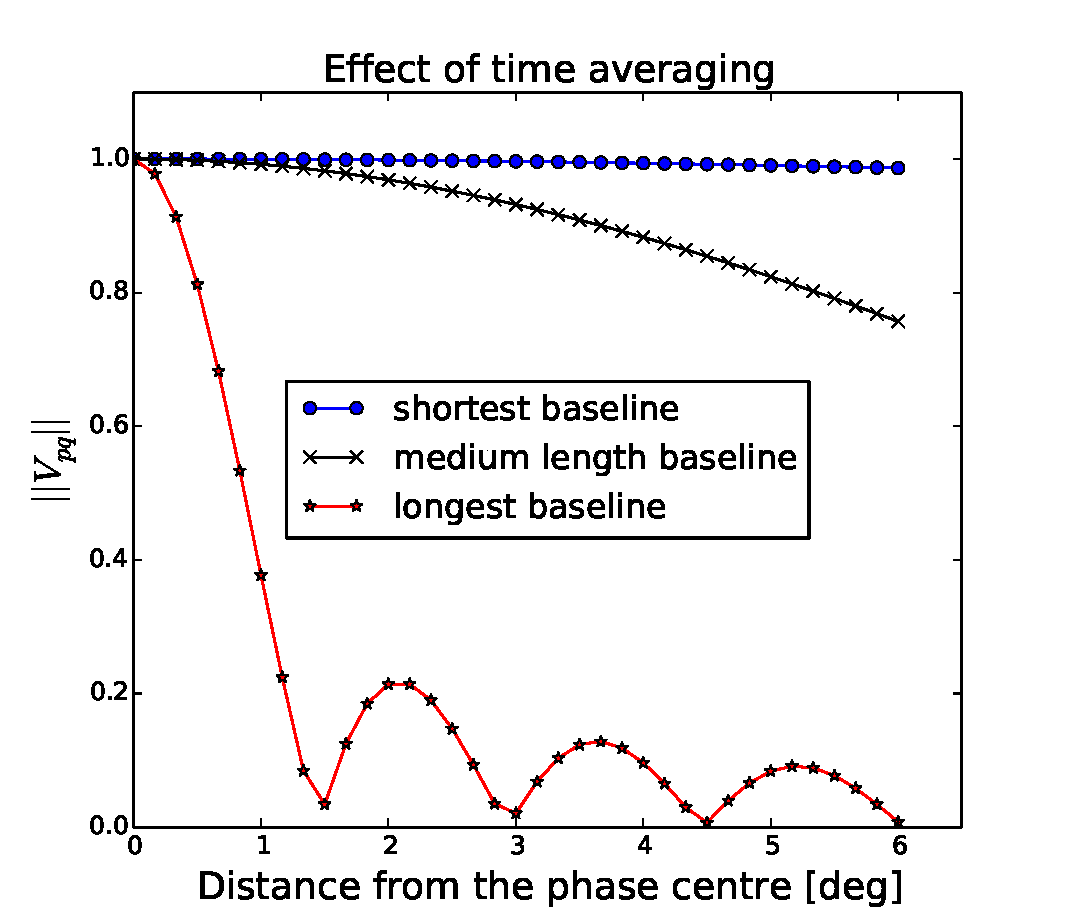
\includegraphics[width=\columnwidth]{./Figures/effect_time_averaging_amplitude.pdf}%
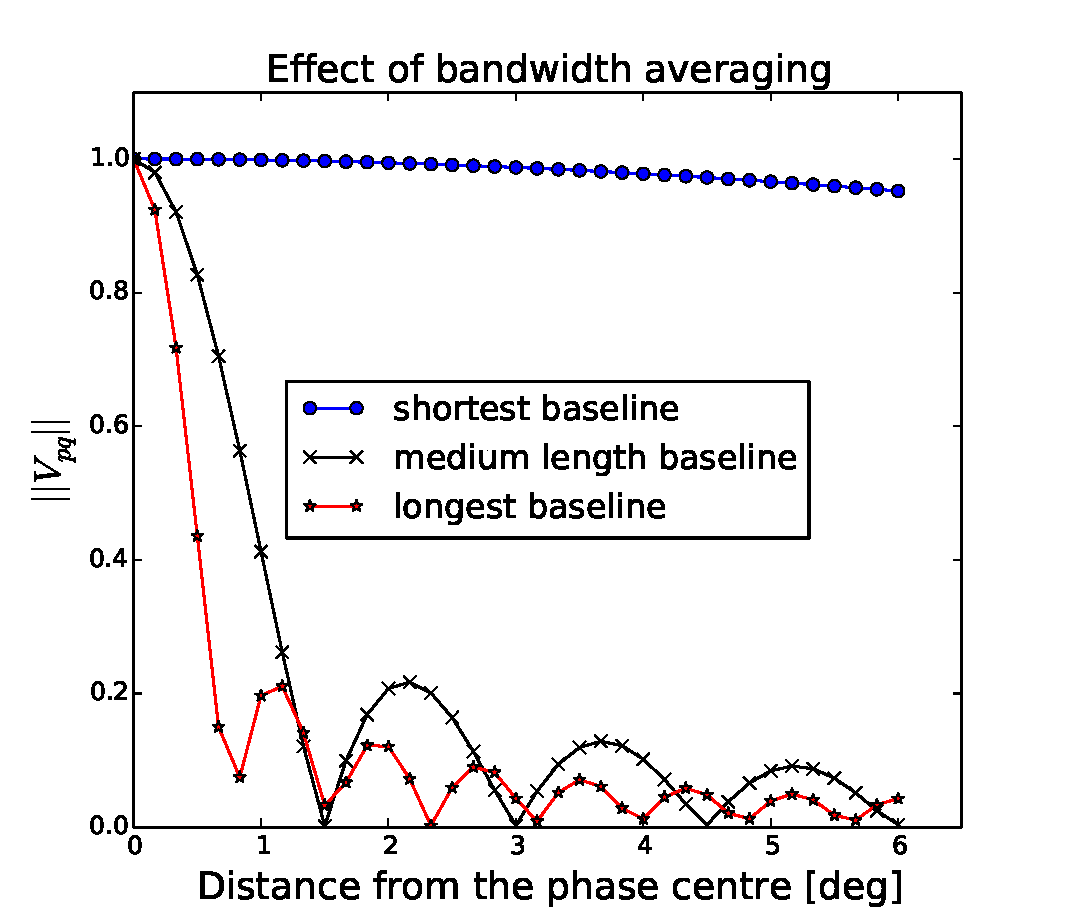
\includegraphics[width=\columnwidth]{./Figures/effect_bandwidth_averaging_amplitude.pdf}
\caption{Amplitude loss: the apparent intensity of a 1 Jy source, as seen by JVLA-C at 1.4 GHz, 
as a function of distance from phase centre. (Left) time and frequency integrations fixed at  100s and 125 kHz respectively; 
(Right) time and frequency integrations fixed at  1 s and 10 MHz respectively.}\label{fig:amplitude}
\end{figure*}


Figure~\ref{fig:srcat30arcmin_avg} shows the amplitude loss as  a function of east-west baseline length. We simulate theBDA source at 
30 arcmin centered at the phase centre and observed the amplitude loss using the JVLA in C configuration.
In this figure, the blue vertical line shows the level of the shortest baseline. In the top panel, the source is
simulated using 100 s integration and 125 kHz channels width, while in the bottom panel the source is simulated using 1 s integration
and 10 MHz channels width.

We observed from  Figure~\ref{fig:amplitude} and Figure ~\ref{fig:srcat30arcmin_avg} that, smearing is severe on  
longer baselines compared to shorter baselines. In addition, the plot 
shows that smearing is also a function of source position in the sky. 

\begin{figure*}
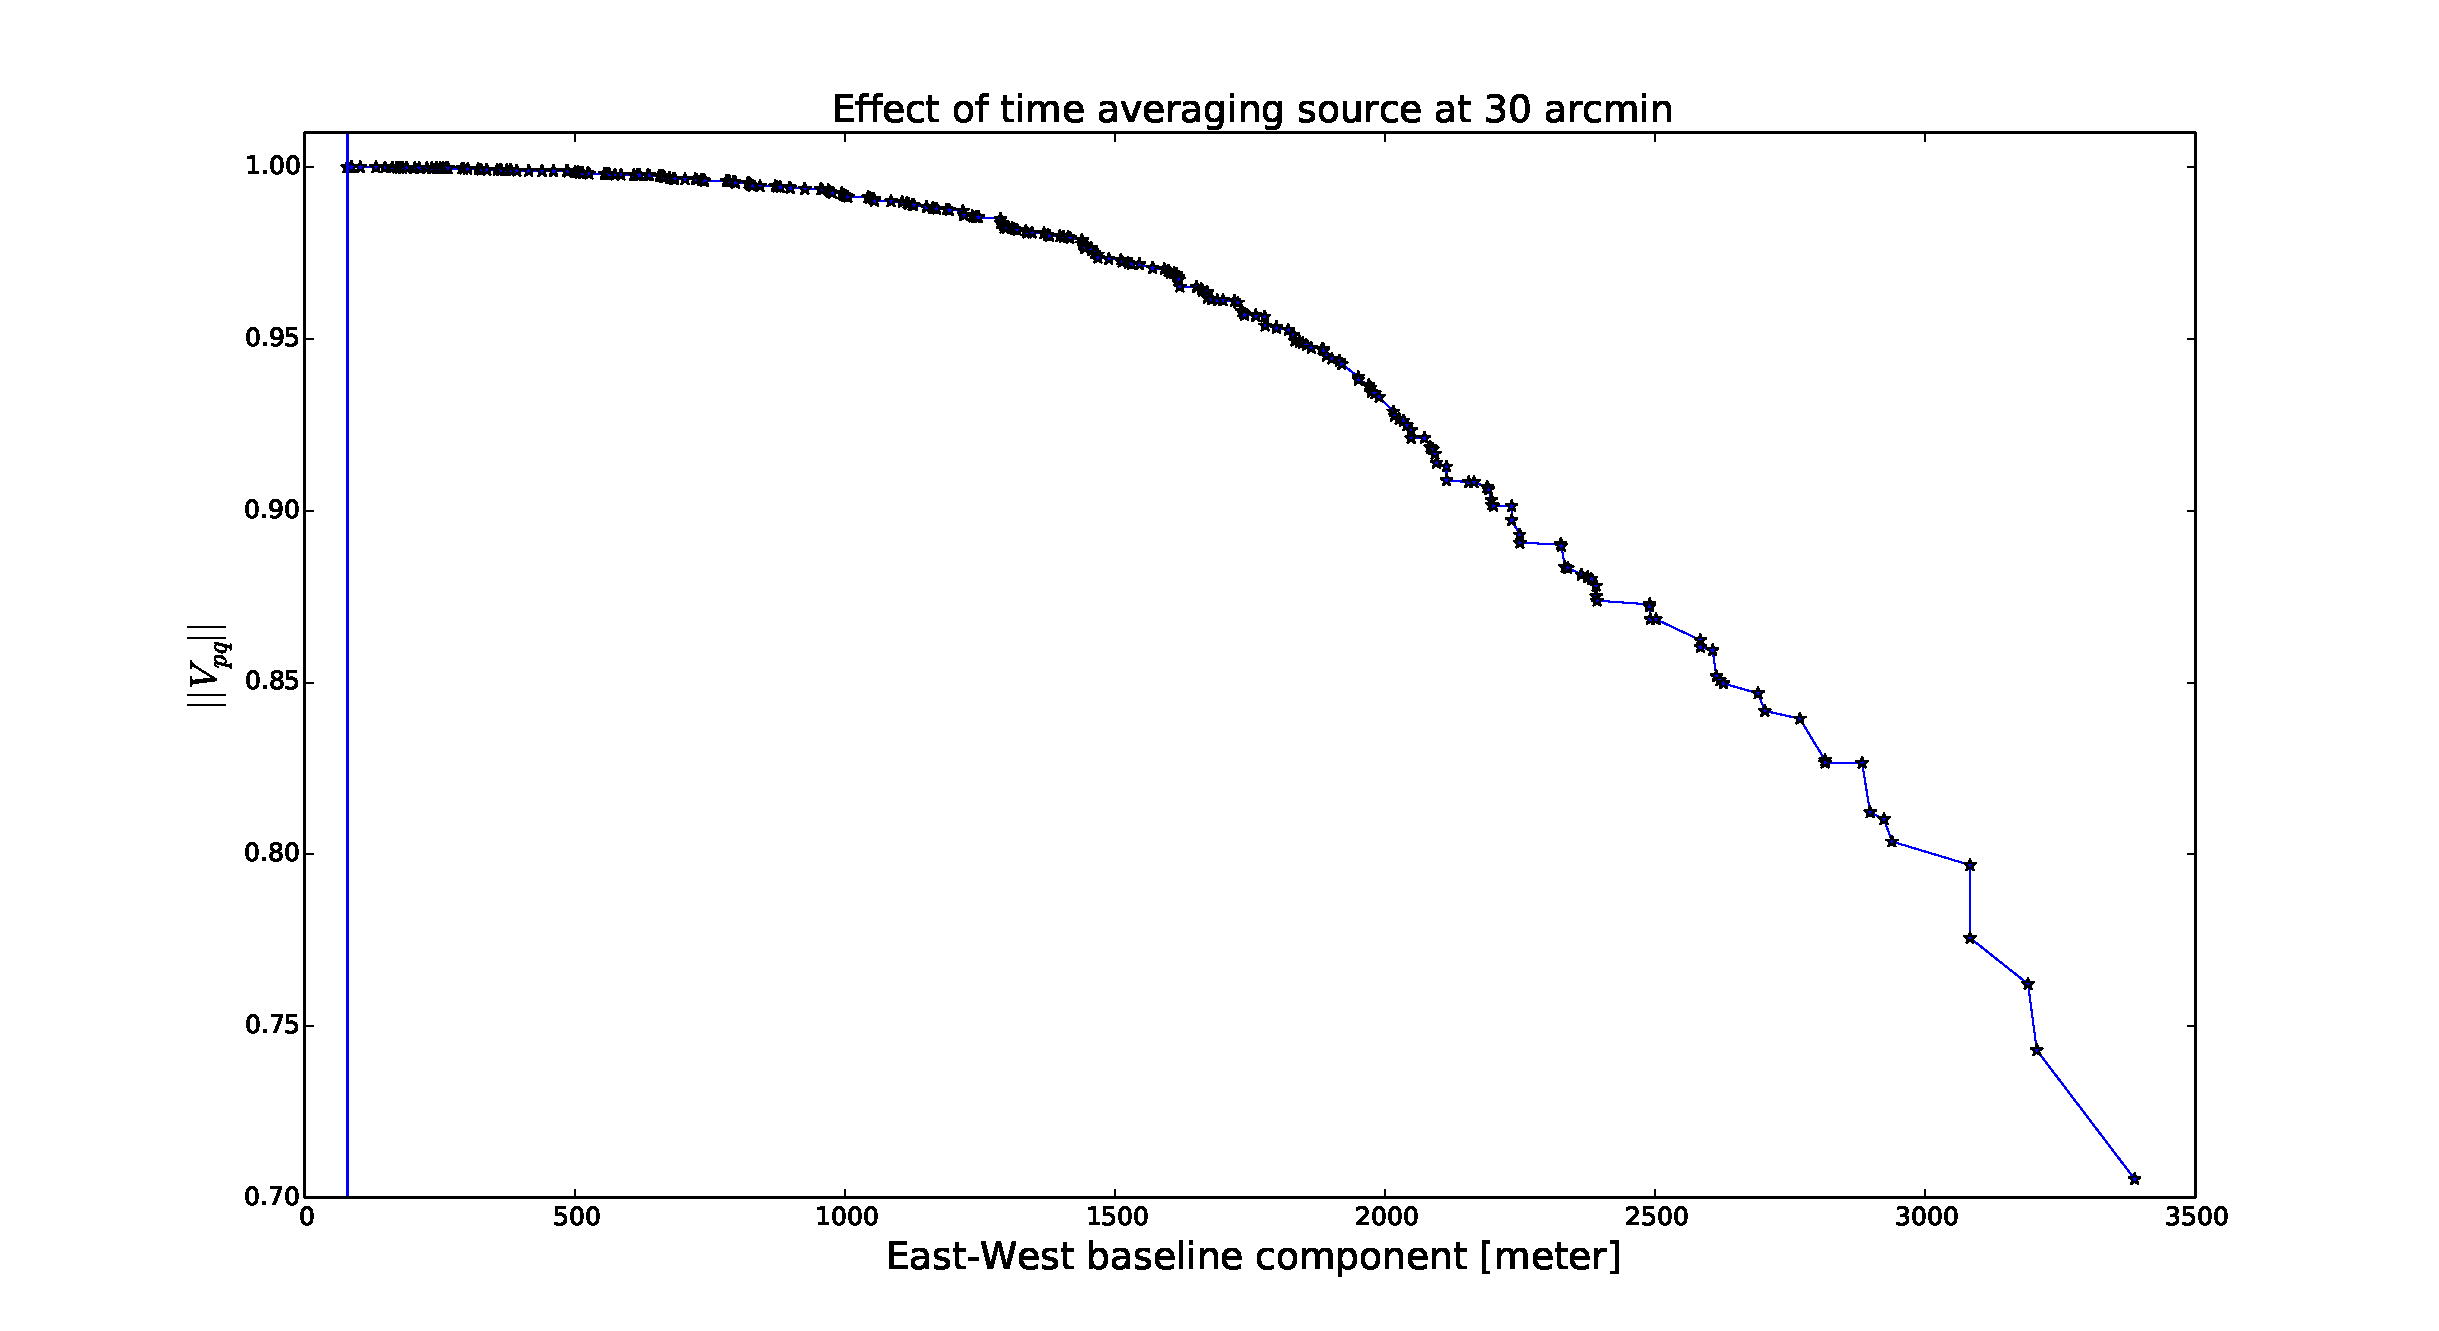
\includegraphics[width=\columnwidth]{./Figures/effect_time_averaging_amplitude_src30arcmin.pdf}%
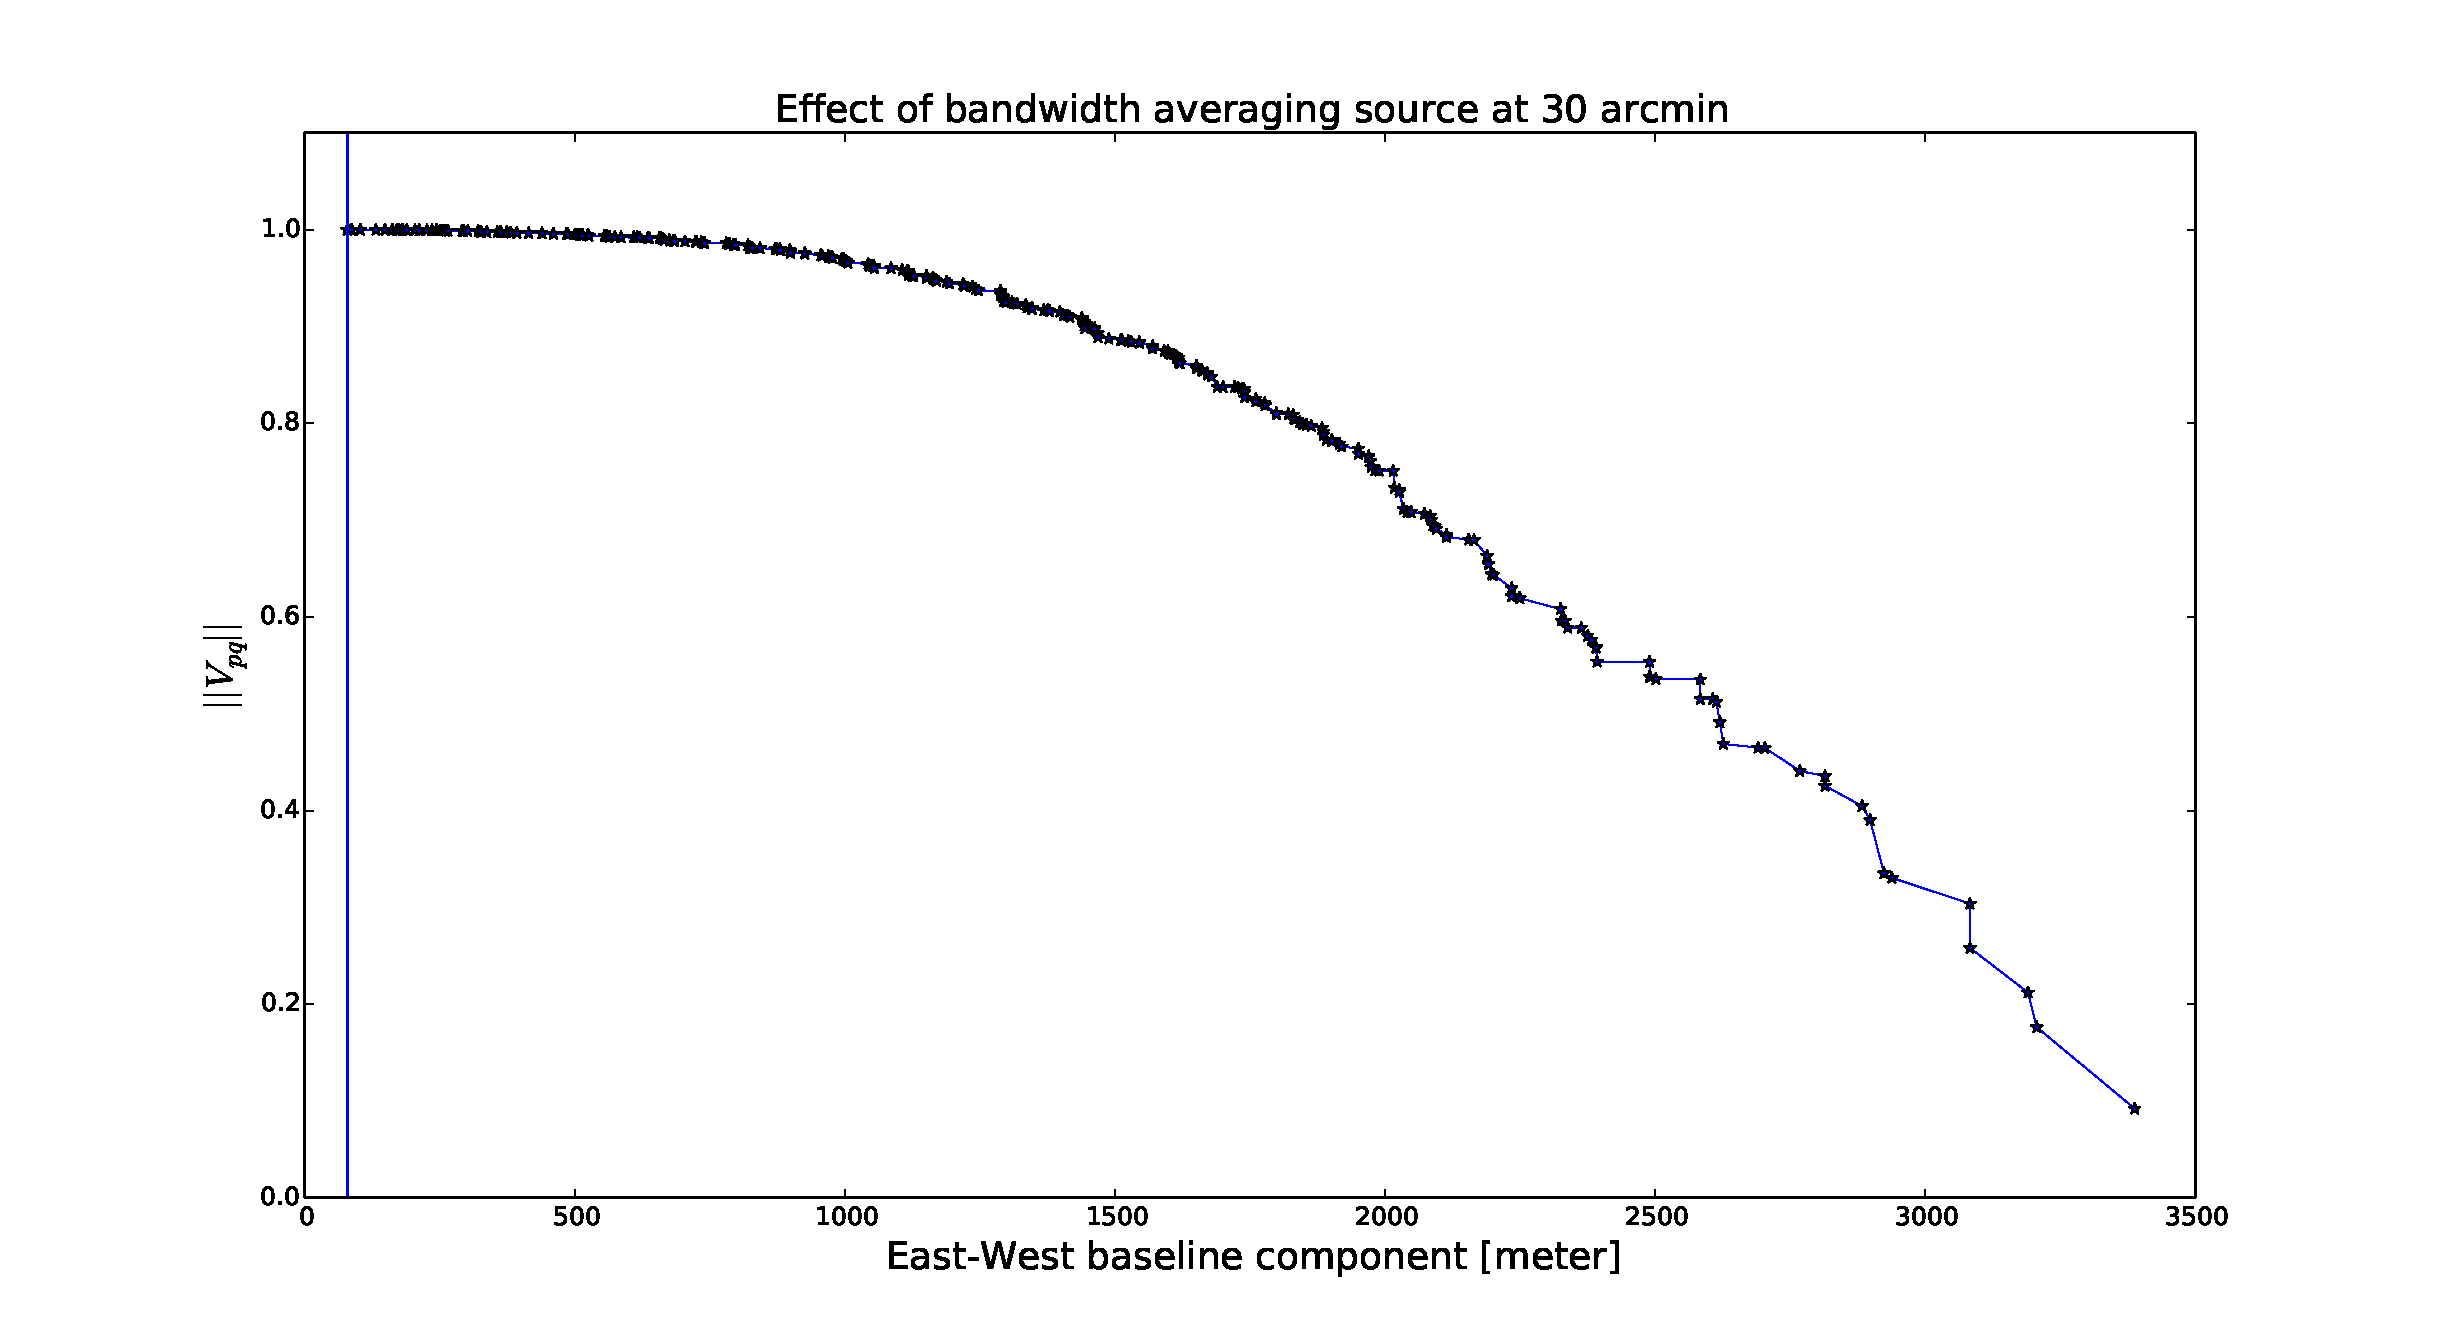
\includegraphics[width=\columnwidth]{./Figures/effect_bandwidth_averaging_amplitude_src30arcmin.pdf}
\caption{Amplitude loss: the apparent intensity of a 1 Jy source, as seen by JVLA-C at 1.4 GHz, 
as a function of Est-West baseline components. (Top) time and frequency integrations fixed at  100s and 125 kHz respectively; 
(Right) time and frequency integrations fixed at  1 s and 10 MHz respectively.}\label{fig:srcat30arcmin_avg}
\end{figure*}

Most of the data measured by any compact interferometer array are from the short baselines. A good illustration is presented in 
Figure~\ref{fig:meerkat}, which is a 1 hour synthesis $uv$-coverage
of the MeerKAT observing at 1.4 GHz. The coverage shows that the data points are more populated in the inner core compared
to the outer core. The data in the inner core are from the short baselines, while the data in the outer core are from the long baselines. 
What if we averaged more samples in the inner core and very little at the outer core? By doing this, 
we avoid smearing
on the longer baselines and compress more data on the shorter baselines. This method 
often referred as \textit{Baseline Dependent Averaging}
was first proposed by \citet{cotton1989special,cotton1999special} as an approach for tackling wide field imaging with little to no
bandwidth and time averaging effects. The next section  describes the mathematical details of BDA.
\begin{figure}
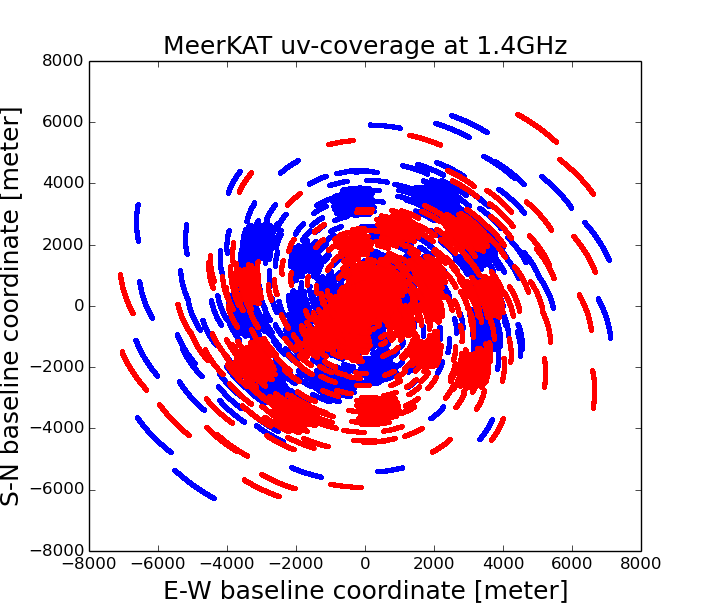
\includegraphics[width=1\columnwidth]{./Figures/uv-coverage-meerkat.png}
\caption{MeerKAT $uv$-coverage at 1.4 GHz, 1 hour observation showing clearly that the data is most 
condensed at the centre core. The data at the inner core are from the shorter baselines, while the data at the outer core
are from the longer baselines.}\label{fig:meerkat}
\end{figure}

\subsection{Baseline Dependent Averaging}
\label{sec:bda}
\begin{figure*}
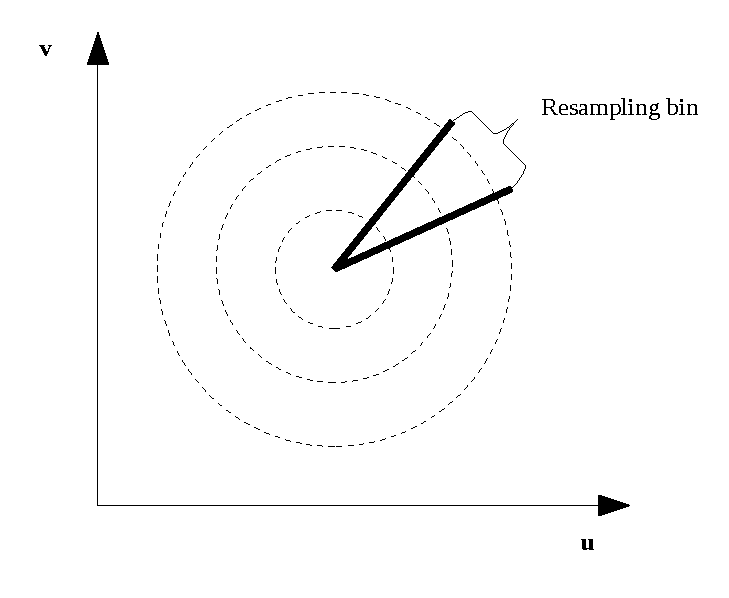
\includegraphics[width=\columnwidth]{./Figures/BDA_design_resamplin_bin_avg.pdf}
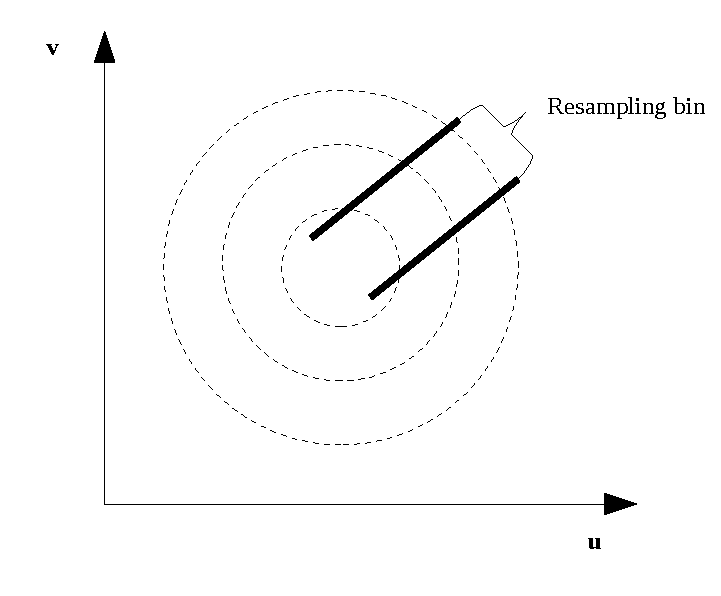
\includegraphics[width=\columnwidth]{./Figures/BDA_design_resamplin_bin_bda.pdf}
\caption{Applying baseline dependent averaging or normal averaging is equivalent to convolving the 
resampling bin by a boxcar windowing function. An Est-West interferometer array, the baseline dependent averaging  (left panel)
 corresponds to an equal convolution kernel and resampling bin across all baselines.}\label{fig:tipical-normalav_bda}
\end{figure*}

Recall from chapter~\ref{chapter3} that an interferometer measures the average visibility over a rectangular time-frequency bin given by the 
time and frequency sampling intervals $\Delta t$ and $\Delta \nu$ respectively, what we called the resampling bin 
(see chapter~\ref{chapter3}, Eq.~\ref{eq:chap3resamplingbin})
\begin{equation}
\Btf_{kl} = \bigg [ t_k-\frac{\Delta t}{2},t_k+\frac{\Delta t}{2} \bigg ]
\times
\bigg [ \nu_l-\frac{\Delta\nu}{2},\nu_l+\frac{\Delta\nu}{2} \bigg ],  
\end{equation}
 where $t_k$ and $\nu_l$ are the centre of $\Delta t$ and $\Delta \nu$ respectively.
 
%  In theBDA case,
%  the sampling interval strictly dependents on the baseline length and direction. 
%  
Let us now define the resampling bin for the case of BDA, where the sampling intervals
 $\Delta t$, $\Delta \nu$ varies across baselines.
 Suppose that the  sampling intervals for a baseline $pq$ are  $\Delta_{pq} t$, $\Delta_{pq} \nu$. We now defined 
 the sampling bin in time and frequency for a baseline $pq$ as follows
 \begin{equation}
\Bda_{kl} = \bigg [ t_k-\frac{\Delta_{pq} t}{2},t_k+\frac{\Delta_{pq} t}{2} \bigg ]
\times
\bigg [ \nu_l-\frac{\Delta_{pq}\nu}{2},\nu_l+\frac{\Delta_{pq}\nu}{2} \bigg ]
\end{equation}
 The resampling bins, 
 $\Bda_{kl}$ is a set of time and frequency bins that  are part of the $uv$-track
 draw by  the baseline $pq$ during the integrations $\Delta_{pq} t$ and $\Delta_{pq}\nu$.
Figure~\ref{fig:tipical-normalav_bda} shows a typical resampling bin for BDA  and the 
resampling bin for simple averaging.

The set of samples $\Bij_{kl}^{pq}$, indexes $ij$ corresponding to the baseline $pq$ \emph{resampling bin}, is given as
\begin{equation}
\Bij_{kl}^{pq} = \big \{ ij:~t_i\nu_j \in \Bda_{kl} \big \},
\end{equation}
Note from this that, if $dim\big\{\Bij_{kl}^{pq}\big\}$, is the number of samples in the resampling bin  then the
baseline sweeps the  distance $\Dbda$ within this sampling bin
\begin{equation}
\Dbda= \sum_{ij \in \Bij_{kl}^{pq}}||\bmath{u}_{pq}(t_i-t_k, \nu_j-\nu_l)||.
\end{equation}
%In the following sections, for simplicity, we will restrict our self to East-West baselines. Note that, 

\begin{figure}
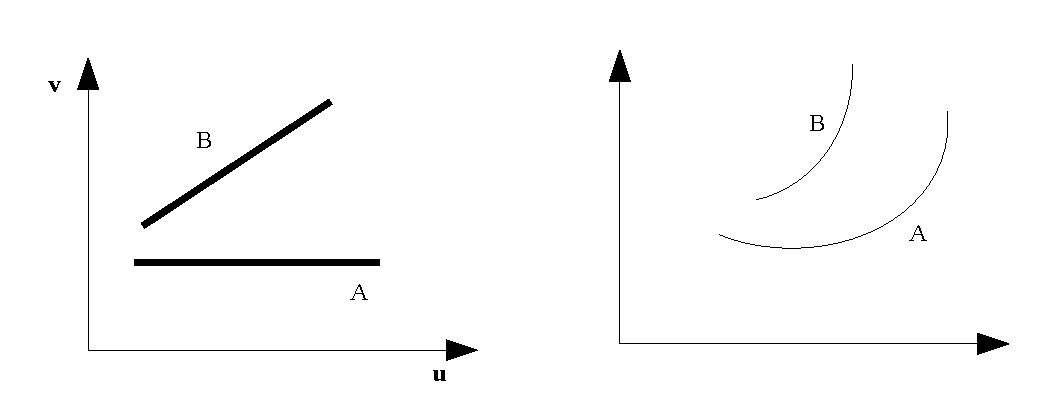
\includegraphics[width=\columnwidth]{./Figures/bda_east_west_two.pdf}
\caption{Two equal lengths baselines A and B with different orientation. The baselne A is a typical
East-West baseline (the South-North component is zero) and B has a non zero South-North and East-West components.
The distances sweep by these baselines
are different during the same time integration.}\label{fig:east_west}
\end{figure}

For simplicity,  we will now refer a baseline from its east-west component. Indeed, all 
baselines have an east-west  and south-north components. During a time/frequency integration, an east-west components has high
rotation speed  compared to the south-north component. The different speeds rate for baselines components indicates that, 
for the same time/frequency integrations, the $uv$-distance sweeps by two equal lengths baselines
oriented differently, may not be equal. This is illustrated
in Figure~\ref{fig:east_west}.

Eq.~(\ref{eq:bda1}) and (\ref{eq:bda2}) must be satisfied for BDA: for all East-West baselines 
$\alpha \beta \neq pq$ with $||\bmath{u}_{\alpha \beta}||\neq ||\bmath{u}_{pq}||$:
\begin{equation}
\Dbdaph=\Dbda \label{eq:bda1}
\end{equation}
\newcommand{\Bdaph}{\mathsf{B}^{[\Delta_{\alpha \beta} t, \Delta_{\alpha \beta} \nu]}}
\begin{equation}
dim \big\{\Bdaph_{kl}\big\} \neq dim \big\{\Bda_{kl}\big\}.label{eq:bda2}
\end{equation}
The above conditions show that, more samples are averaged on the shorter baselines compared to the longer baselines.
For example, suppose $p=1$, $q=2$ are the indexes for the longest baseline and $p=2$, $q=3$ the indexes for the 
medium length baseline
and $p=3$, $q=4$ the indexes for the shortest baseline. If these three baselines are East-West baselines or 
East-West components, we have
\newcommand{\Dbdlong}{\mathsf{D}^{[\Delta_{12} t, \Delta_{12} \nu]}}
\newcommand{\Dbdmedium}{\mathsf{D}^{[\Delta_{23} t, \Delta_{23} \nu]}}
\newcommand{\Dbdshort}{\mathsf{D}^{[\Delta_{34} t, \Delta_{34} \nu]}}
\newcommand{\Bdaphlong}{\mathsf{B}^{[\Delta_{12} t, \Delta_{12} \nu]}}
\newcommand{\Bdaphmedium}{\mathsf{B}^{[\Delta_{23} t, \Delta_{23} \nu]}}
\newcommand{\Bdaphshort}{\mathsf{B}^{[\Delta_{34} t, \Delta_{34} \nu]}}
\begin{equation}
\Dbdlong=\Dbdmedium\\
	=\Dbdshort\\
dim \big\{\Bdaphlong_{kl} \big\}< dim \big\{\Bdaphmedium_{kl}\big\} \\
		    <dim \big\{\Bdaphshort_{kl}\big\}.
\end{equation}
The averaged intervals are function of baselines length and direction, with longer baselines having shorter integration time and
narrower channels width, while on the other hand, shorter baselines are averaged over longer integration time and wider channels widths.

Recall that in chapter~\ref{chapter3} (section~\ref{sec:AvgCon}), we defined the averaged 
or \emph{resampled} visibilities for a baseline $pq$ as  the discrete sum
\begin{equation}
\label{eq:discrete:bdaavg}
V^\mathrm{(m)}_{pqkl} = \frac{1}{n_{pq}} \sum_{ij\in\Bij_{kl}^{pq}}  \Vs_{pqij},
\end{equation}
where  $dim\big\{\Bij_{kl}^{pq}\big\}= n_{pq}$ is the number of samples that has been averaged. It was  then 
shown that averaging is a convolution at the centre  of the resampling bin interval
\begin{equation}
V^\mathrm{(m)}_{pqkl} = [ \VV_{pq} \circ \Puv_{pq} ](\bmath{u}_{pq}(t_k,\nu_l)),
\label{eq:avscon}
\end{equation}
and this results to Eq.~(\ref{eq4:imagetaaper}), when 
imaging the per-baseline visibilities:
\begin{equation}
\IID =  \sum_{pqkl} W_{pqkl} \PP_{pqkl} \circ (\II\cdot\TT_{pq}),~~\TT_{pq}=\FF^{-1}\{ \Puv_{pq} \}.\label{eq4:imagetaaper}
\end{equation}

Now let us see what Eq.~(\ref{eq4:imagetaaper}) becomes with BDA. For BDA, the $uv$-space boxcar windows $\Puv_{pq}$,
are approximately equal across all baselines and therefore, not any more a function of baseline length and/or direction. In 
other words,  
for any baseline $\alpha\beta\neq pq$, $\Puv_{\alpha\beta} \approx \Puv_{pq}$. This derivation, 
 $\Puv_{\alpha\beta} \approx \Puv_{pq}$ is valid and correct, but one thing to keep in mind. Although the size of all boxcar windows are the same in $uv$-space for BDA, but they are sampled differently.
The  boxcar window are well sampled
on the shorter baselines compared to the longer baselines, and which may result in
different image plane taper. 

However, 
if the pre-averaged visibilities are sampled at  significantly  high time and
spectral resolution, then we can assume that all these boxcar at different baseline are sampled equaly.
Taking this assumption into account,  we can write
%in such a way that, the sampling rate is approximately equal on all baselines, then we can write
\begin{equation}
\TT_{pq}\approx \TT_{\alpha\beta },
\end{equation}
 which shows that, the time and bandwidth smearing represent the effect of a single taper in the image.
 With this condition, Eq.~(\ref{eq4:imagetaaper}) becomes
\begin{equation}
\IID \sim  \sum_{pqkl} W_{pqkl} \PP_{pqkl} \circ \II\cdot\TT_{}, \label{eq:bda2}
\end{equation}
where $\TT_{}\approx \TT_{pq}\approx \TT_{\alpha\beta }$ is the smearing response, constant on all baselines.


\subsection{Compression factor}
The compression factor is defined as the ratio between the pre-averaged  data (high-res data) size and the average data (low-res data) size.
If a complex value is stored with 32 bits,  the data size of the high-res measurement set is defined as
\begin{equation}{2}
Data~size~hires   = \frac{N\times(N-1)}{2}\times N_{sub}  \times N_{tslt}^{hires} \times N_{ch}^{hires}\times N_{pol}\times 32 ~[bits]
,\label{eq:memorychap4hires}
\end{equation}
where  $N$ is the number of antennas of the interferometer array, $N_{sub}$ the number of 
sub-bands, $N_{pol}$ is the number of polarizations, $N_{tslt}^{hires}$ and $N_{ch}^{hires}$ are the number
of timeslots and channels of the high-res  measurement set respectively. 
In the case of simple averaging, the data size of the average measurement set is given by
\begin{equation}
Data~size~avg = \frac{N\times(N-1)}{2}\times N_{sub}  \times \frac{N_{tslt}^{hires}}{n_t} \times \frac{N_{ch}^{hires}}{n_{\nu}}\times N_{pol}\times 32 ~[bits],\label{eq:memorychap4}
\end{equation} 
where $n_t$ is the number time bins and  $n_{\nu}$ is the channels  averaged on each baseline.
Note that this formulation applies for an equal compression across all baselines, therefore the compression factor is defined by
\begin{equation}{2}
Compression~factor~avg = \frac{Data~size~hires}{Data~size~avg}\\
		      =n_t\times n_{\nu}
\end{equation} 
The space savings which is defined as the reduction in size relative to the high-res data size therefore follows
\begin{equation}{2}
space~savings~avg = 1-\frac{Data~size~avg}{Data~size~hires}\\
		      =1-\frac{1}{n_t\times n_{\nu}}
\end{equation} 
% of antennas of the interferometer array, $N_{sub}$ the number of sub-bands, $T_{obs}$ is the observation time, 
% $B_{w}$ is the total bandwidth, $N_{pol}$ is the number of polarizations, $\Delta t$ and $\Delta \nu$
% the sampling intervals. The quantities, 
% $ N_{tslt}^{avg}=T_{obs}/\Delta t $ and $N_{ch}^{avg}=B_{w}/\Delta \nu$ are the number of timeslots and channels of the averaged dataset respectively. 
% 
% If $N_{tslt}^{hires}$ and $N_{ch}^{hires}$ are the number of timeslots and channels of the pre-averaged dataset (the hires resolution dataset)
% then $N_{tslt}^{avg}=N_{tslt}^{hires}/n_t $ and $N_{ch}^{avg}=N_{ch}^{hires}/n_{\nu}$, where $n_t$ and $n_{\nu}$ are the number of samples
% in the sampling intervals.
% Eq~\ref{eq:memorychap4} shows that each baseline has a  compression factor of $n_t\times n_{\nu}$, therefore the interferometer array
% compression factor is given as
% \begin{equation}
% Comp\_factor = \frac{N\times(N-1)}{2}n_t\times n_{\nu}.
% \end{equation} 
Let us now define the compression factor for BDA. Recall that in this case, the compression rate
varies across baselines.  Following
the analogy for BDA resampling bins, the number of samples in the resampling bin for 
a baseline $pq$ is defined as $dim\Bda_{kl}=n_{t}^{pq}\times _{\nu}^{pq}$, where $n_{t}^{pq}$ and $n_{\nu}^{pq}$ are
the number of time and frequency samples respectively. The interferometer array data size for BDA then follows 
\begin{equation}{2}
 Data~size~bda =\sum_{pqkl} N_{sub}  \times \frac{N_{tslt}^{hires}\times N_{ch}^{hires}}{dim\{\Bij_{kl}^{pq}\}} \times N_{pol}\times 32 ~[bits]\\
	  =\sum_{pq} N_{sub}  \times \frac{N_{tslt}^{hires}}{n_{t}^{pq}} \times \frac{N_{ch}^{hires}}{n_{\nu}^{pq}}\times N_{pol}\times 32 ~[bits]
,\label{eq:memorychap4bd}
\end{equation}
% We previously defined  $dim\Bij_{kl}^{pq}$, as the number of time samples $n_{t}^{pq}$, and the number of frequency samples 
% $n_{\nu}^{pq}$ in the resampling bin $\Bij_{kl}^{pq}$ of the  baseline $pq$, thus $dim\Bij_{kl}^{pq}=n_{t}^{pq}\times n_{\nu}^{pq}$. \\
% % We can write
% \begin{equation}{2}
% DataSize   &=\sum_{pq} N_{sub}  \times \frac{N_{tslt}^{hires}\times N_{ch}^{hires}}{n_{t}^{pq}\times n_{\nu}^{pq}} \times N_{pol}\times 32 ~[bits]
% \end{equation}
The interferometer array compression factor for BDA is then given by
\begin{equation}{2}
Compression~factor~bda  =\frac{N(N-1)}{2}\times \Bigg(\sum_{pq} \frac{1}{n_t^{pq}\times n_{\nu}^{pq}}\Bigg)^{-1},\label{compresionbdafactor}
\end{equation} 
and the space savings is
\begin{equation}{2}
space~savings~bda   =1-\Bigg(\frac{N(N-1)}{2}\Bigg)^{-1}\times \sum_{pq} \frac{1}{n_t^{pq}\times n_{\nu}^{pq}}
\end{equation} 
In the rest of this chapter, we refer to compression factor as $CF=x_{t}\times y_{\nu}$, where $x_t$ is the compression factor in time 
and $y_{\nu}$ is the compression factor in frequency. The notation, $CF=x_{t}\times 1$ implies the data is 
compressed only in time by a factor of $x_{t}$, while $CF=1\times y_{\nu}$ implies that  data is  compressed only in frequency
 by a factor of $y_{\nu}$.

\section{Implementation details}
\label{BDA:impl}
The principal difficulty with BDA is that, the visibility plane contains either repeatedly averaged values or 
flagged data points. The correlation matrix is a  time and frequency regular grid.
Averaging entries in this correlation matrix
over long times for  short baselines and short times for  long baselines result to an irregular grid.  
In practice, a better idea is to map this irregular
correlation matrix onto a regular grid by either
flagging out the supplementary points, or duplicating the averaged values on these supplementary points.
We explain these processes in the following. 
\subsection{Flagging}
In the BDA procedure, one has to make sure  that the resampling bin interval contains an 
odd number of data points in time and frequency i.e,
\begin{equation}
dim \big\{\Bdaph_{kl}\big\}=(2k_t+1)(2k_{\nu}+1), ~~ k_t ~~ and ~~ k_{\nu} ~~ are~ integers
\end{equation}
where $2k_t+1$ is the 
number of visibilities to average in time and $2k_{\nu}+1$ the number of visibilities to average in frequency.  
This condition must hold on all baselines otherwise the average
baseline vector may not coincide with the mid time and frequency vector and will lead to a phase shift. 
If this condition is satisfied,
the average value is assigned to the mid resampling bin interval point i.e at the $k_t^{th}+1$ and $k_{\nu}^{th}+1$ visibility point. The 
others entries of the resampling bin are assigned a flag value which is generally unity. 
This flag  value will account for missing samples during  post-processing. 
Let us suppose that the data in Figure~\ref{fig:bdavgflagging} represents 15 time-bins,  for three different baselines i.e
the longest, the medium length and a shortest baseline.
Each bin is a 1 s integration sample and  15 s bins are averaged on the shortest baseline, 
5 s    on the medium length baseline and 
3 s on the longest baseline. The colored pointers indicate the averaged bins and the black pointers the flagging points. 
Note that most of the flagging occurs on the shortest baselines because of the larger time bins averaged (15 s).
\begin{figure}
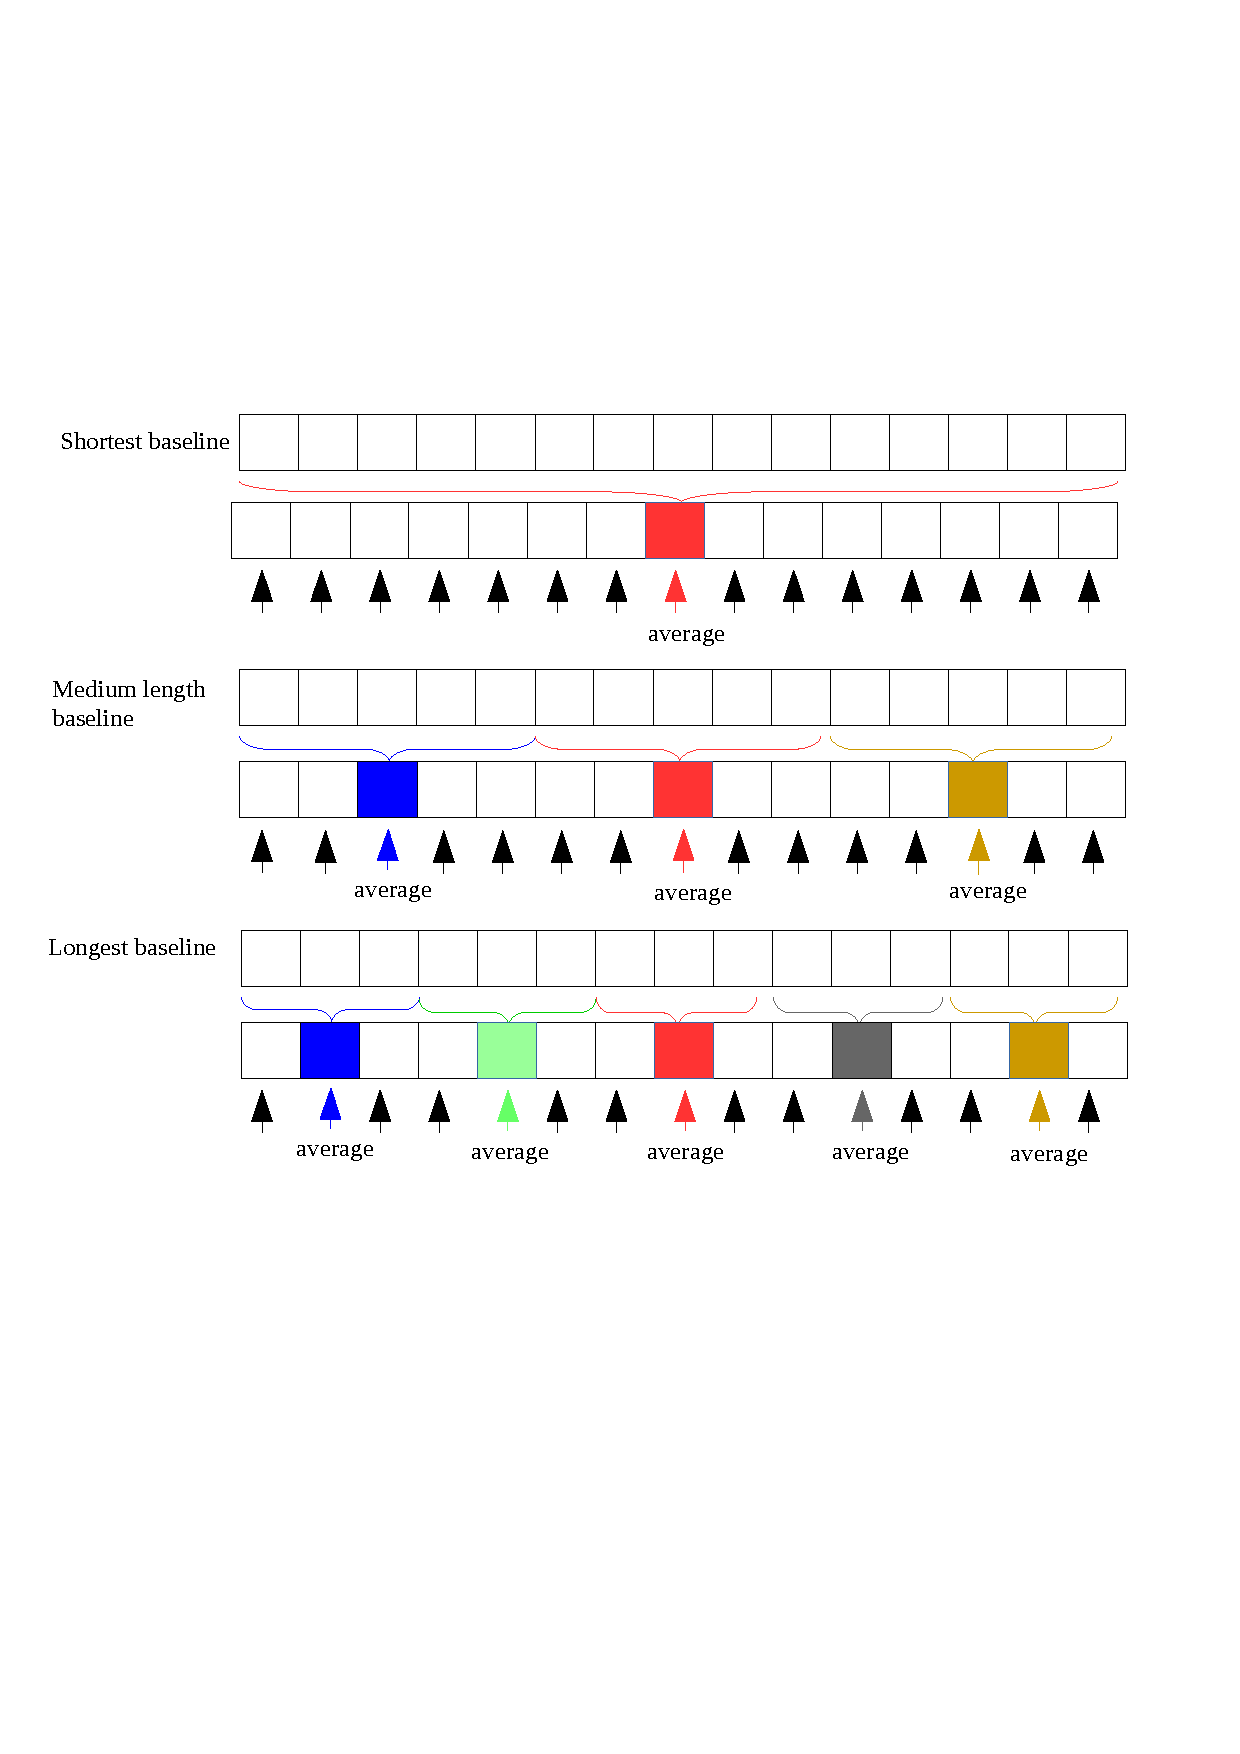
\includegraphics[width=\columnwidth]{./Figures/bda_averaging_senario.pdf}
\caption{Baseline dependent averaging with flagging: the bins are averaged and the average
value is assign at the centre of the resampling bin interval, while a flagging value is assign to others points.}\label{fig:bdavgflagging}
\end{figure}
% \begin{itemize}
%   \item On the shortest baseline, all the 15 time bins are averaged and the average value is assign 
% to the mid bin i.e at the bin number 7, the red pointer indicates this point. A flag value is affected to any other bins (the black pointers
% indicate these points).
%   \item On the medium length baseline, each block of 5s time bins are averaged and this average value is assign 
% to the mid bin of each block i.e at the bin number 3, 8 and 13, the red pointers indicate these points. 
% A flag value is affected to the other bins (the black pointers indicate these points).
%   \item On the shortest baseline, all the 15 time bins are averaged and the average value is assign 
% to the mid bin i.e at the bin number 7, the red pointer indicates this point. A flag value is affected to any other bins (the black pointers
% indicate these points).
% \end{itemize}
\subsection{Duplication}
This method consists of duplicating the average value at all entries of the resampling bins. While this process is 
easier to implement than the flagging method, it may not serve the purpose of data compression  and/or 
quick computation for post-processing. Easier to implement in the sense that, one may not care or always verify that the
number of visibilities points in the resampling bin is an odd number. Also note here that the data size of the resulting
measurements set remains the same as the pre-averaged measurement set due to the fact that all value were duplicate along 
the pre-averaged measurement set.
This method may be used in practice for cases where one does not want to average the uv coordinates
as there are in the pre-averaged measurement set. While this  method may be of little use, it is interesting due to the fact that 
its leads to an increased in nominal sensitivity since averaging represents  maximum sensitivity.
% In addition to an increased in sensitivity, we show
%  that this is more than made up for by a decrease in smearing over the rest of the FoV. 
 Similarly to the example in Figure ~\ref{fig:bdavgflagging}, 
 Figure~\ref{fig:bdavgduplication} represents the duplicate method. Pointers with the same color indicate 
 the duplicate averaged values throughout the 
resampling bin intervals.
\begin{figure}
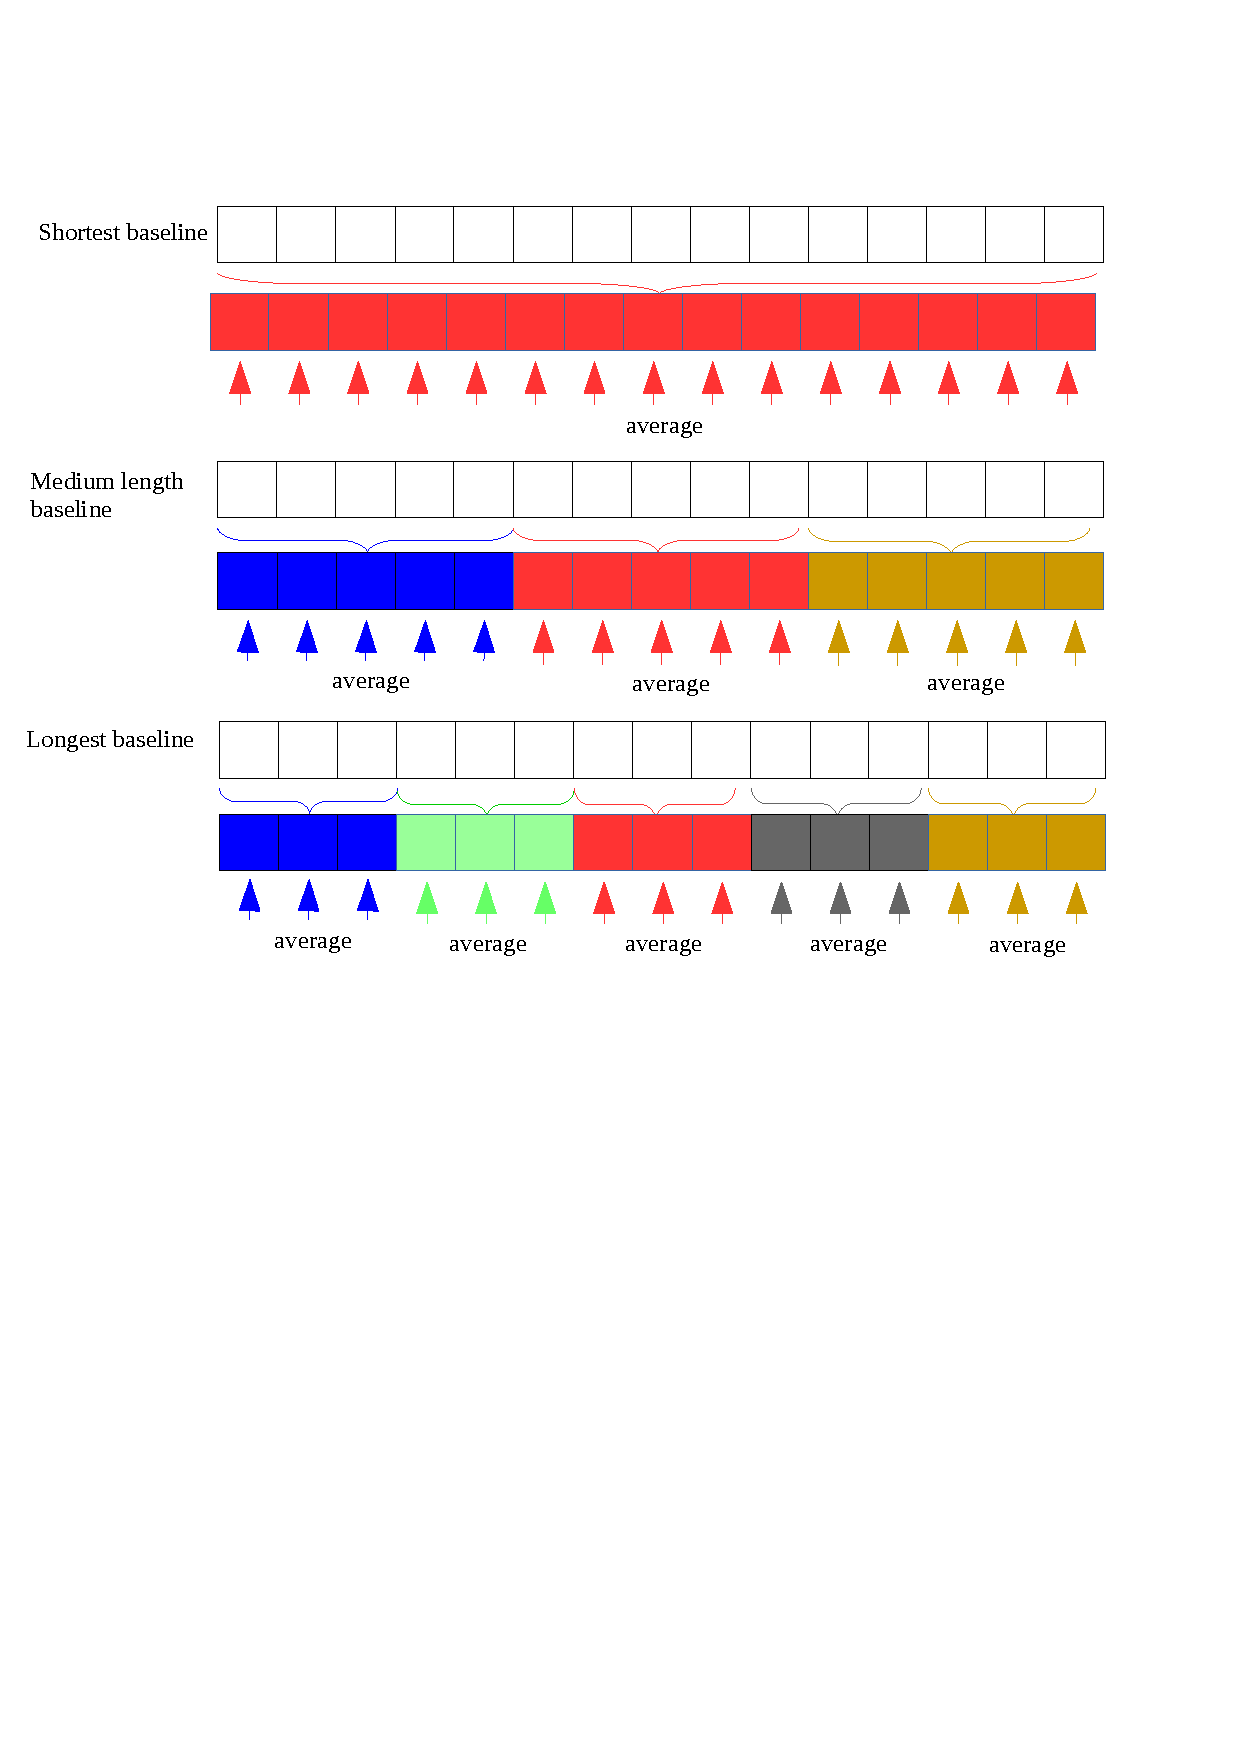
\includegraphics[width=\columnwidth]{./Figures/bda_averaging_duplication_senario.pdf}
\caption{Baseline dependent averaging with duplication: the bins are averaged and the average
value is assign at all points of the resampling bin interval.}\label{fig:bdavgduplication}
\end{figure}
\subsection{Semi duplication and flagging}
This method consists of combining the flagging and the duplicate methods in other to benefit  of their full  advantages.
 By so doing, we seek both for data compression and  quick computation while on the other hand, the implementation is easier to
 handle. 
We have learned from the flagging method that it is complex to implement but save for data compression and quick processing. 
We also learned from the duplication method that its does not help for compression or quick data processing but easier to implement. The semi duplication and flagging method should be able to account for both data compression aspects and easier implementation simultaneously.
The idea is to duplicate the averaged bin along two central entries of the resampling bin if the total number of 
entries within this resampling bin is even otherwise the averaged bin is assigned only on the central bin of the resampling
bin. Any other entry is then flagged as we shall learn in the example presented in Figure~\ref{fig:bdavgsimeduplicationflagging}. 
\begin{figure}
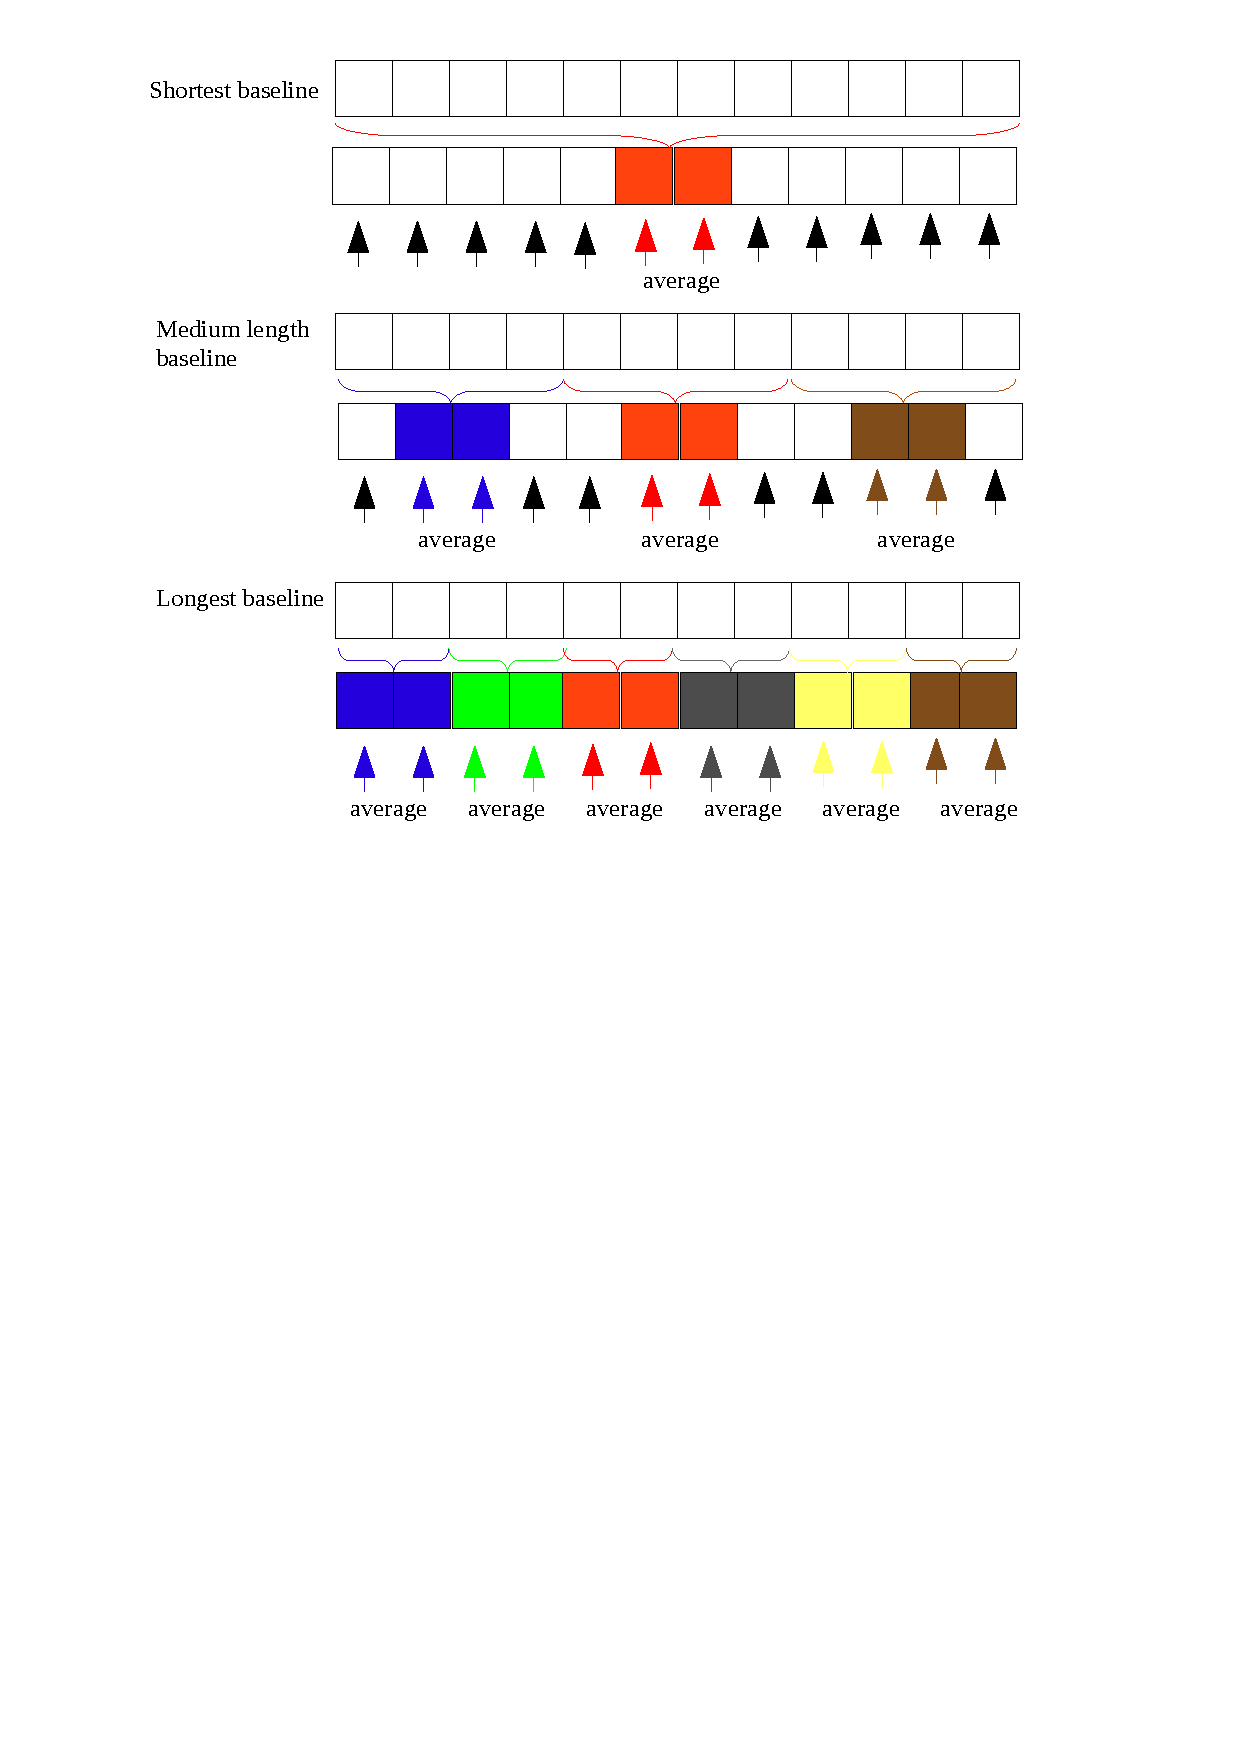
\includegraphics[width=\columnwidth]{./Figures/bda_averaging_semi_duplication_flaggin_senario1.pdf}
\caption{Baseline dependent averaging with semi duplication and flagging: the bins are averaged and the average
value is duplicated only at the two central points of the resampling bin interval and the other bins are flagged.}\label{fig:bdavgsimeduplicationflagging}
\end{figure}

\section{Simulations and results} 

Having explored the mathematics and difficulties behind  the implementation  of BDA,
we now turn to the simulation aspects. To probe the simulation issue, we consider our tests
on a sky model of 1 Jy point source at various sky positions,  with no noise or other corruptions included.
Using the JVLA telescope in its C configuration, we evaluate the efficiency of a BDA correlator using 
two different procedure. First, we simulate the source at a fixed sky position and applied BDA, and measured 
the averaging effects separately on each baselines. Second, we simulate the point source  at various radius from the phase 
centre and applied BDA, and BDWFs across equal $uv$-distance, hereby  evaluating the interferometer array 
cumulative smearing effects on all baselines. 
Following the same procedure used in chapter~\ref{chapter3} (section~\ref{chap3:simulation}), we measured the source 
peak amplitude in each image after averaging. Since each dirty image corresponds to a single source, the peak gives
us the degree of smearing associated with a given averaging method and compression factor.

\subsection{Source amplitude vs east-west baseline length} 
We simulate two high-res measurement sets each with a source at 30 arcmin from the phase centre of the observation.
Furthermore, we generates two low-res measurement sets to receive the resampled visibilities. We present the amplitude loss 
as a function of Est-West baseline length.
The results of  BDA and simple averaging are compared in Figure~\ref{fig:srcat30arcminx}. 
 \begin{itemize}
  \item The first dataset from which the results are presented 
 in the top panel of Figure~\ref{fig:srcat30arcminx} consisted of 10 frequencies
 channels of 125 kHz width for high spectral resolution, and
 1000 timeslots of 1 s integration time.  
 In this test, the  compression factor is fixed to 48 both for BDA and simple averaging.
  Note that, for  BDA, the shorter baselines are compressed by a lot more than 48 while the longer baselines
 by a lot less, this correspond to  4 s on the longest baseline and 250 s on the shortest baseline, while 
 for simple averaging, 48 s bins are averaged in time. 

  \item The second dataset consists of 10 timeslots of 1s integration, and
 1000 frequencies channels of 125 kHz bins width.  The compression factor is fixed to 32 both for BDA and simple averaging.
 For BDA, this result to 100kHz and 11kHz averaging bins in frequency for the shortest and the longest baseline respectively, 
 while 30kHz frequencies bins are averaged for simple averaging.
\end{itemize}
It is  pretty noticeable in Figure~\ref{fig:srcat30arcminx} that on shorter baselines, the smearing rate of  
BDA and simple averaging are equivalent. The physical interpretion of this is that, at this compression rate, 
visibilities averaging do not suffer from decorrelation on the shorter baselines. On the other hand,  BDA suppresses smearing 
on the longer baselines compared to simple averaging. This is because fewer samples are averaged on the longer baselines 
when applying BDA, thereby causing a decrease in decorrelation.


\begin{figure}
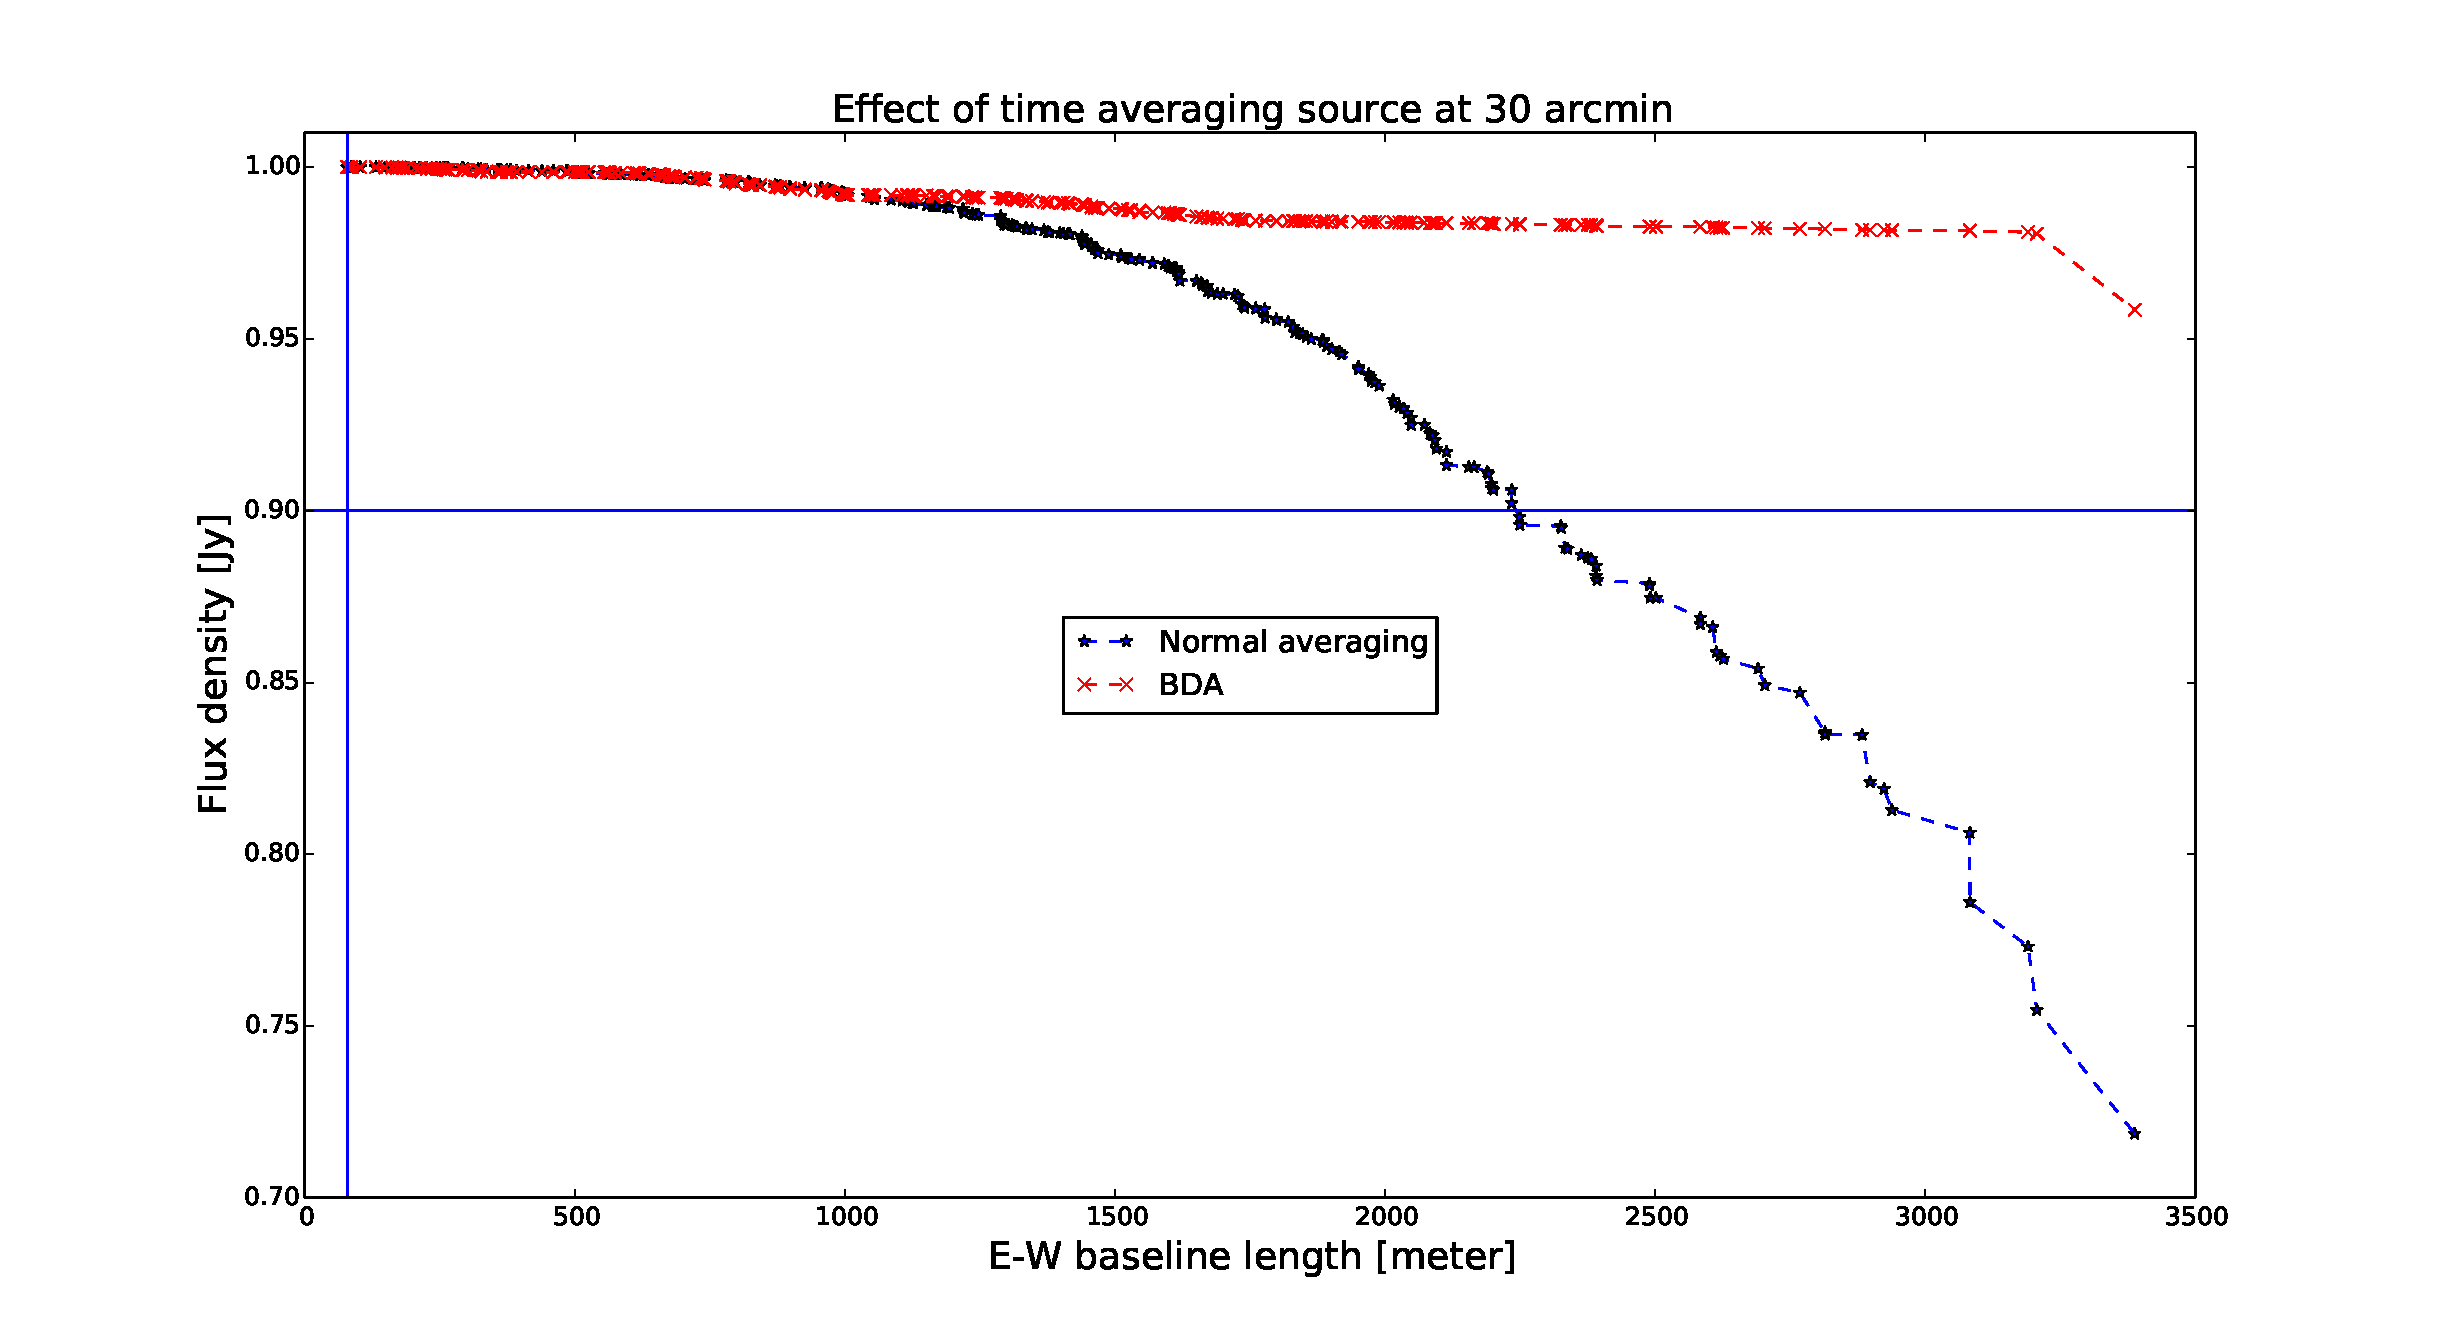
\includegraphics[width=\columnwidth]{./Figures/time_bda_navg.pdf}\\
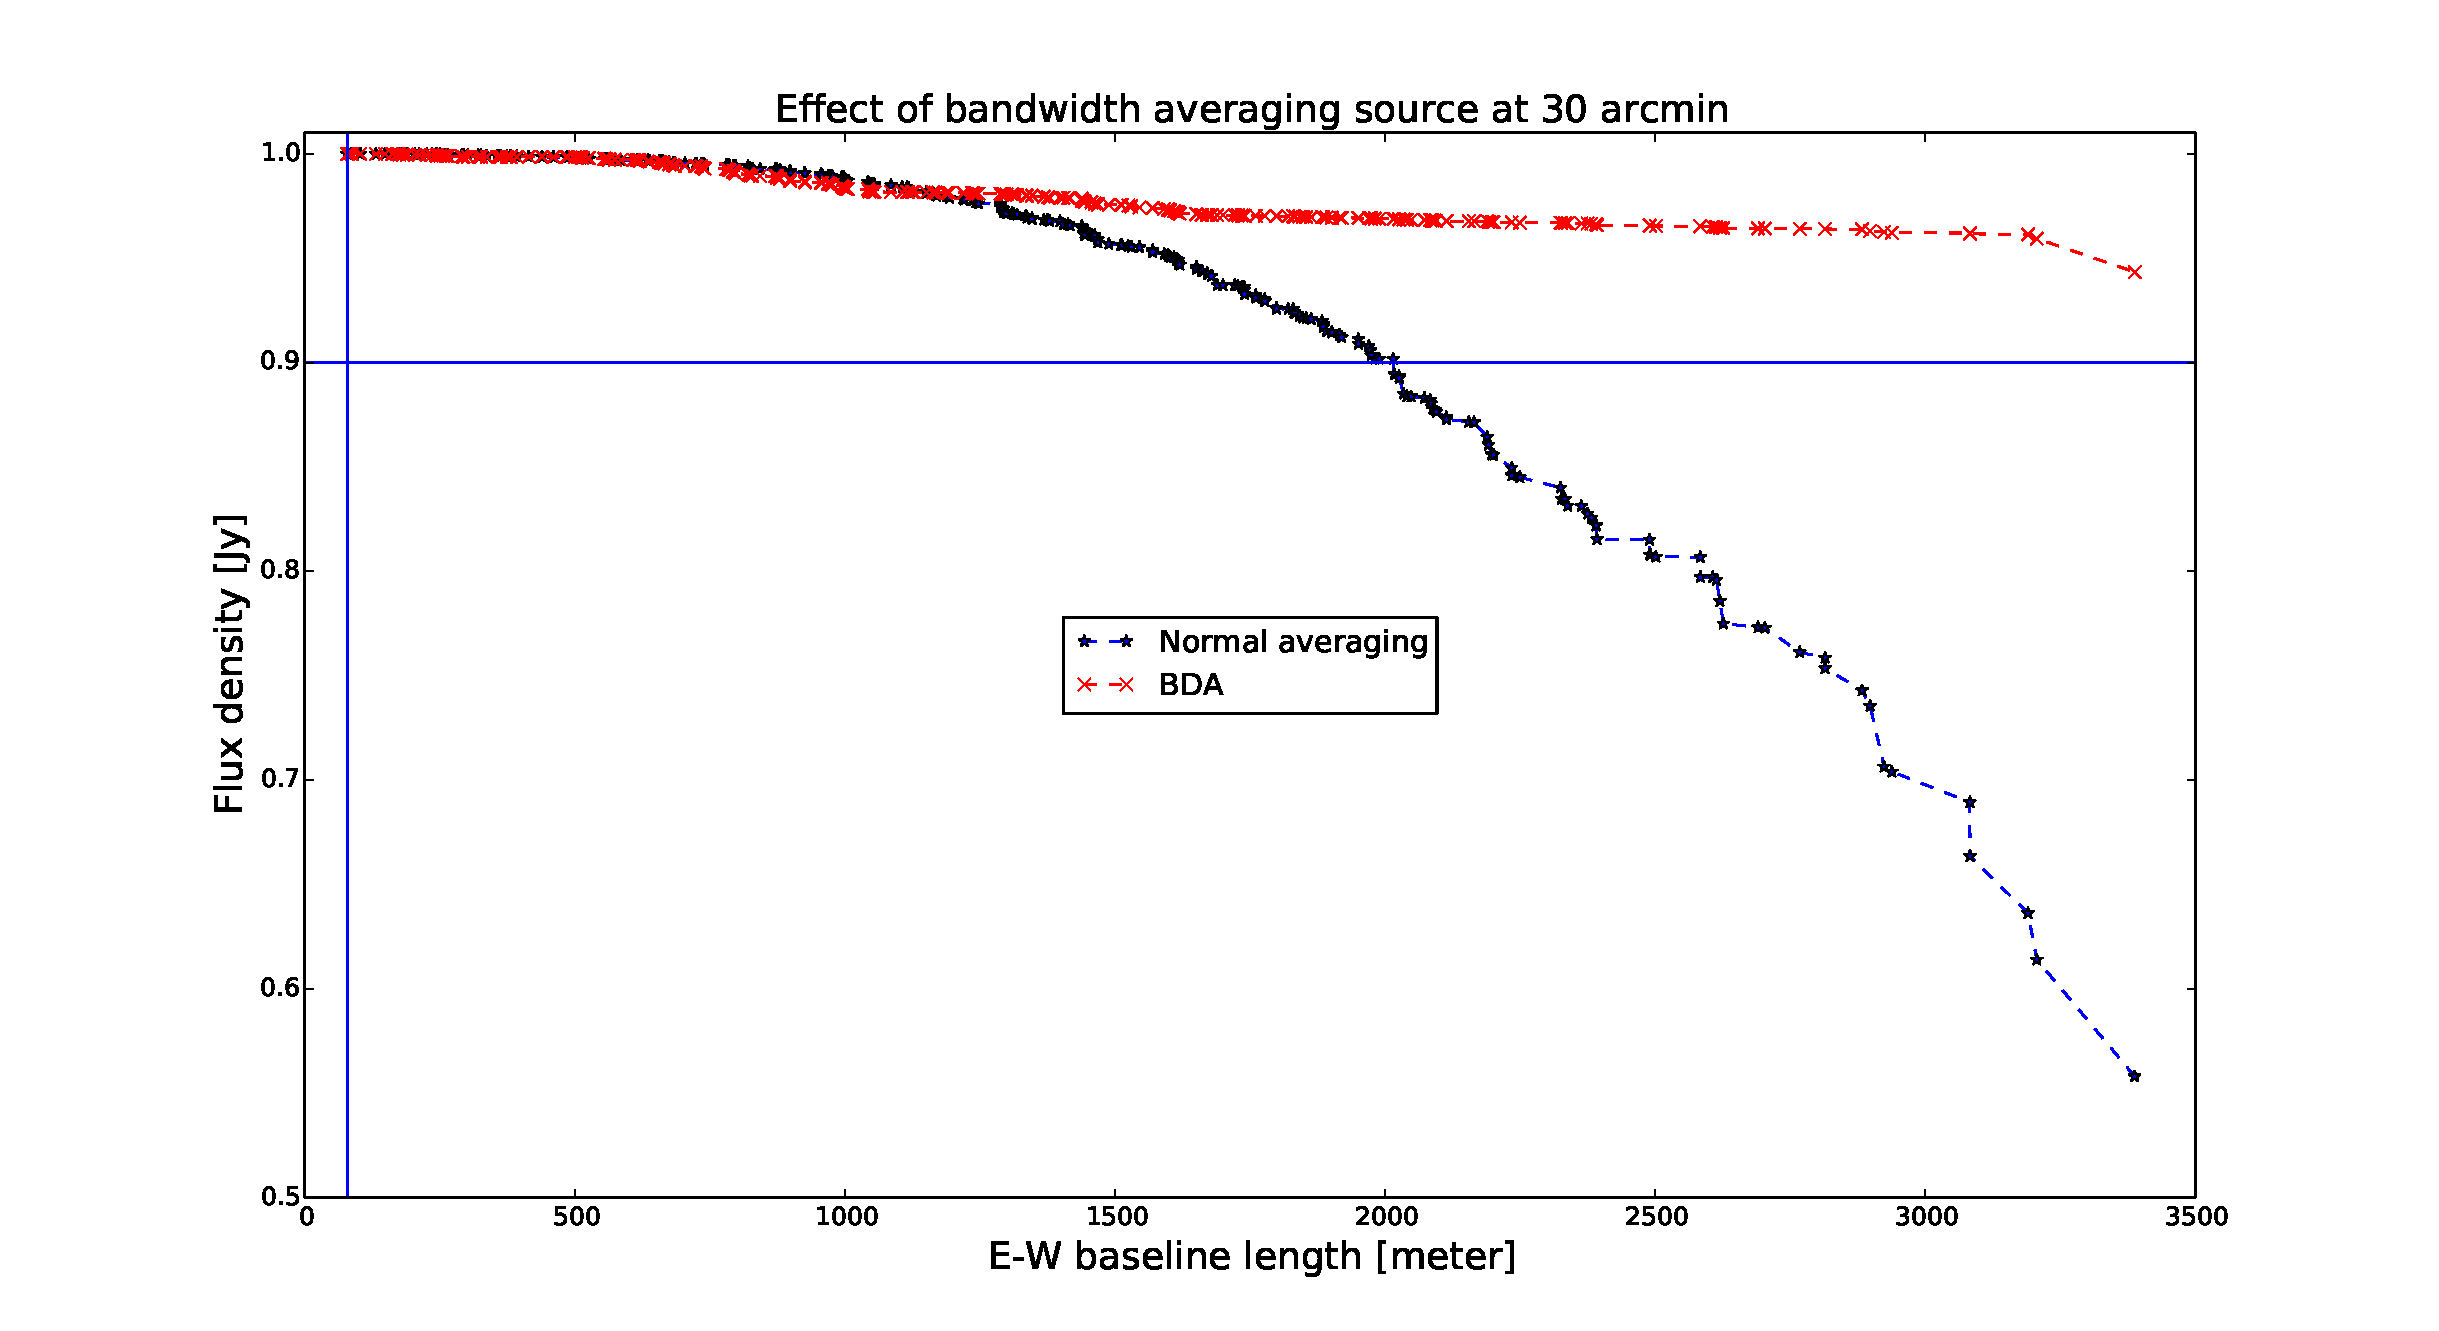
\includegraphics[width=\columnwidth]{./Figures/bandwidth_bda_navg.pdf}
\caption{Amplitude loss: the apparent intensity of a 1 Jy source, as seen by JVLA-C at 1.4 GHz, 
as a function of Est-West baseline components. (Top) time and frequency integrations fixed at  100s and 125 kHz respectively; 
(Right) time and frequency integrations fixed at  1 s and 10 MHz respectively.}\label{fig:srcat30arcminx}
\end{figure}

\subsection{Source amplitude vs distance from the phase centre}

In this section, we simulate a high-res measurement set corresponding to a 
375 s synthesis at 1 s integration, with 42.6 MHz total bandwidth
centred  at 1.4 GHz, divided into 511 channels of 83.4 kHz each. The sky model is a single 1 Jy point source at 
a given distance from the phase centre with noise free. We then generate two measurement sets to receive the 
resampled visibilities:
 \begin{enumerate}[(a)]
  \item A low-res measurement set to receive the resampled visibilities with simple averaging. This measurement set correspond to 
  25 s integration time and 2.5 MHz channels width. I remind the reader that, the synthesis time for this measurement set is
  325 s splitted into 13 timeslots with  37.5 MHz total bandwidth divide into 15 channels each of width 2.5 MHz.
  It is pretty remarkably that, the synthesis time and the total bandwidth are less than the hight-res measurement set.
  We learned from chapter~\ref{chapter3} (section~\ref{baseline2}) that, for overlap BDWFs some number of time and frequencies bins must
  be allowed at the observation starting time/or frequency and ending time and/or frequency. These overlapping bin correspond
  here  to 50 s and 2.5 MHz in time and frequency respectively.
  \item The second measurement set is prepared to receive the sampled visibilities for BDA. This MS is a copy of the hight-res MS where 
    one of the BDA implementation methods describe in section~\ref{BDA:impl} will be apply. It is important to note here that,
    for the case of overlap BDWFs, all the bins reserved for the overlap filters will be flagged at the end of the resampled 
    procedure i.e before the resampled visibilities are imaged.
\end{enumerate}
% Based on the above discussion, we can now interpret some our main results.
% % \subsubsection{ BDA vs normal averaging}
% % For the first set of simulations, the low-res MSs corresponds to a 
% % 
% % \begin{figure}[h!]
% % \hspace{-1.8cm}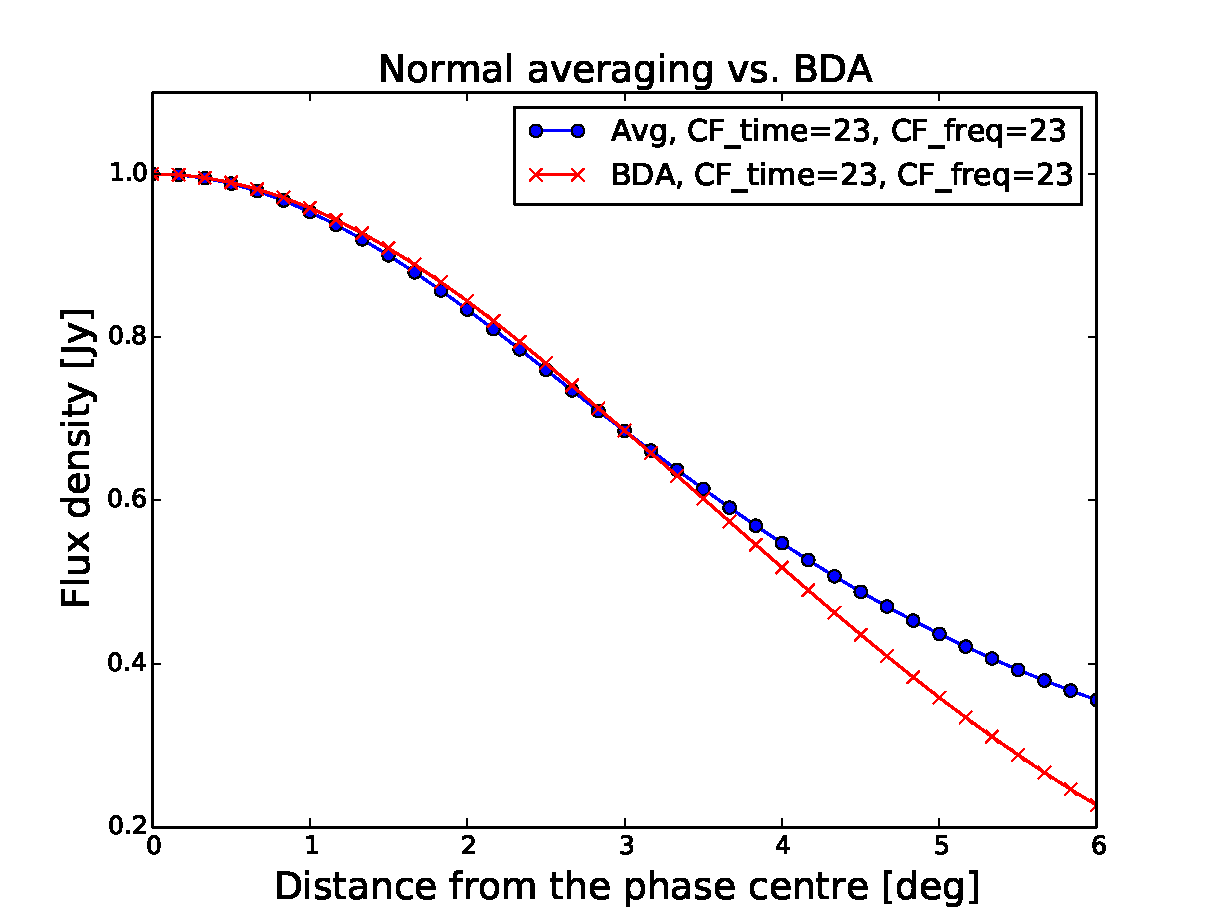
\includegraphics[width=1.5\textwidth, angle =90 ]{./Figures/NormalAVG_BDA_23s_23MHZ.pdf}
% % \caption{Amplitude loss: the apparent intensity of a 1 Jy source, as seen by JVLA-C at 1.4 GHz, 
% % as a function of Est-West baseline components. (Top) time and frequency integrations fixed at  100s and 125 kHz respectively; 
% % (Right) time and frequency integrations fixed at  1 s and 10 MHz respectively.}\label{fig:srcat30arcmin}
% % \end{figure}
% % 
% 
% The results show that the effect of amplitude loss is proportional across all baselines and still depend on the source location.veraging and BDA are compared 
% 
% Remarkably, this equation shows that the effect of elastic fluctuations is to decrease, at
% any given t (in the high-temperature regime), the minimum value of H0 required for the
% appearance of real-space oscillatory decay of C
% G. The physical reason is that the timepersistent
% random strain fields created by the random, relaxational, displacements of the
% volume elements of the elastomer after the instant of cross-linking enhance the effective
% disorder strength, thereby making it easier for the translational aggregation mechanism to
% % occur (and also make it harder for nematogens to align via local rotations).
% 
% \subsubsection{BDWFs applies across equal uv distance vs normal averaging} 
As was discussed in chapter~\ref{chapter3} (section~\ref{sec:baselinewfs}), applying BDWFS to visibilities 
also results in different image plane tapers. For example, with 
a \WF{sinc}{1}{1}, 
longer baselines correspond  to sinc-like window function and boxcar taper in the image plane. 
While  for shorter baselines, a \WF{sinc}{1}{1} correspond to boxcar and a sinc-like taper in the image plane, and therefore increased
smearing. Applying BDA to BDWFS may lead to a more optimal response given that the shorter baselines and the longer
baselines are adapted with the same visibility plane sinc-like convolution kernel, 
thus resulting to an equal boxcar taper in the image plane.

To distinguish the case of overlapping BDWFs applied across an equally $uv$-distance from non-overlapping ones, 
we will designate the overlapping window functions  as $bda$-$WF$-$x \times y$. It implies that, for  all 
baselines, $x$ s and  $y$ MHz bins are overlap in time and frequency respectively. For example,
$bda$-$sinc$-25$\times$ 2.5 is an overlap baseline dependent sinc function applies across an equal $uv$-distance, and where 
the total bins averaged are ($25 + \Delta_{pq} t$) s and $(2.5 + \Delta_{pq} \nu$) MHz in time and frequency respectvely.
%\newcommand{\BIN}[2]{#1s$\times$#2MHz}

The compression factor for the results presented in this section is fix to $CF$=25$\times$30 for
for all averaging methods i.e for simple averaging, 25 and 30 time and frequency bins are averaged in time
and frequency respectively. For BDA, the averaged time and frequency bins are baseline dependent as presented
in Appendix~\ref{AppendixC}.

In Figure \ref{fig:bda-sn-bessel-2ge}, 
we compare the performance of simple averaging with a resampling bin sizes 
of \BIN{25}{2.5} (solid grey lines) to:

 \begin{itemize}
  \item $bda$ (solid red lines), which is a BDA with a compression factor 
  equal to $CF$=25$\times$30 
  \item An overlapping $bda$-$sinc$-25$\times$ 2.5 turned over two FoVs, $2\circ$ (solid blue lines) 
  and $4\circ$ (dashed blue lines)
  \item An overlapping $bda$-$bessel$-25$\times$ 2.5 turned over two FoVs, $2\circ$ (solid green lines) 
  and $4\circ$ (dashed green lines)
\end{itemize}


Based on the above discussion, we can now interpret some our main results. 
This results can be alternatively appreciated by regarding the performances of BDWFs apply across 
an equal  $uv$-distance on all baselines. 

\begin{enumerate}[(a)]
\item BDA provides good results in flux recovery i.e for $5\%$ smearing, this gives us
a field with radius $1.4^{\circ}$ while with simple averaging, we can only recover a field with radius $0.9^{\circ}$  at this compression
factor. We can also notice from the result that, BDA is far to achieve source suppression.
\item Overlapping BDWFs apply across equal uv-distance ($bda$-$sinc$-25$\times$ 2.5, $bda$-$bessel$-25$\times$ 2.5)
performance is excellent for  source suppression and flux recovery within the choosing FoV.
 If the desired FoV size is $2^{\circ}$ or $4^{\circ}$, overlapping BDWFs ($bda$-$sinc$-25$\times$ 2.5,
$bda$-$bessel$-25$\times$) provide excellent performance (1\% or less) compared to
averaging, the smearing performance
across the FoV is  better than that of simple averaging or BDA, and out-of-FoV source suppression 
is almost two orders of magnitude higher.
 \end{enumerate}

\begin{figure}
\centering
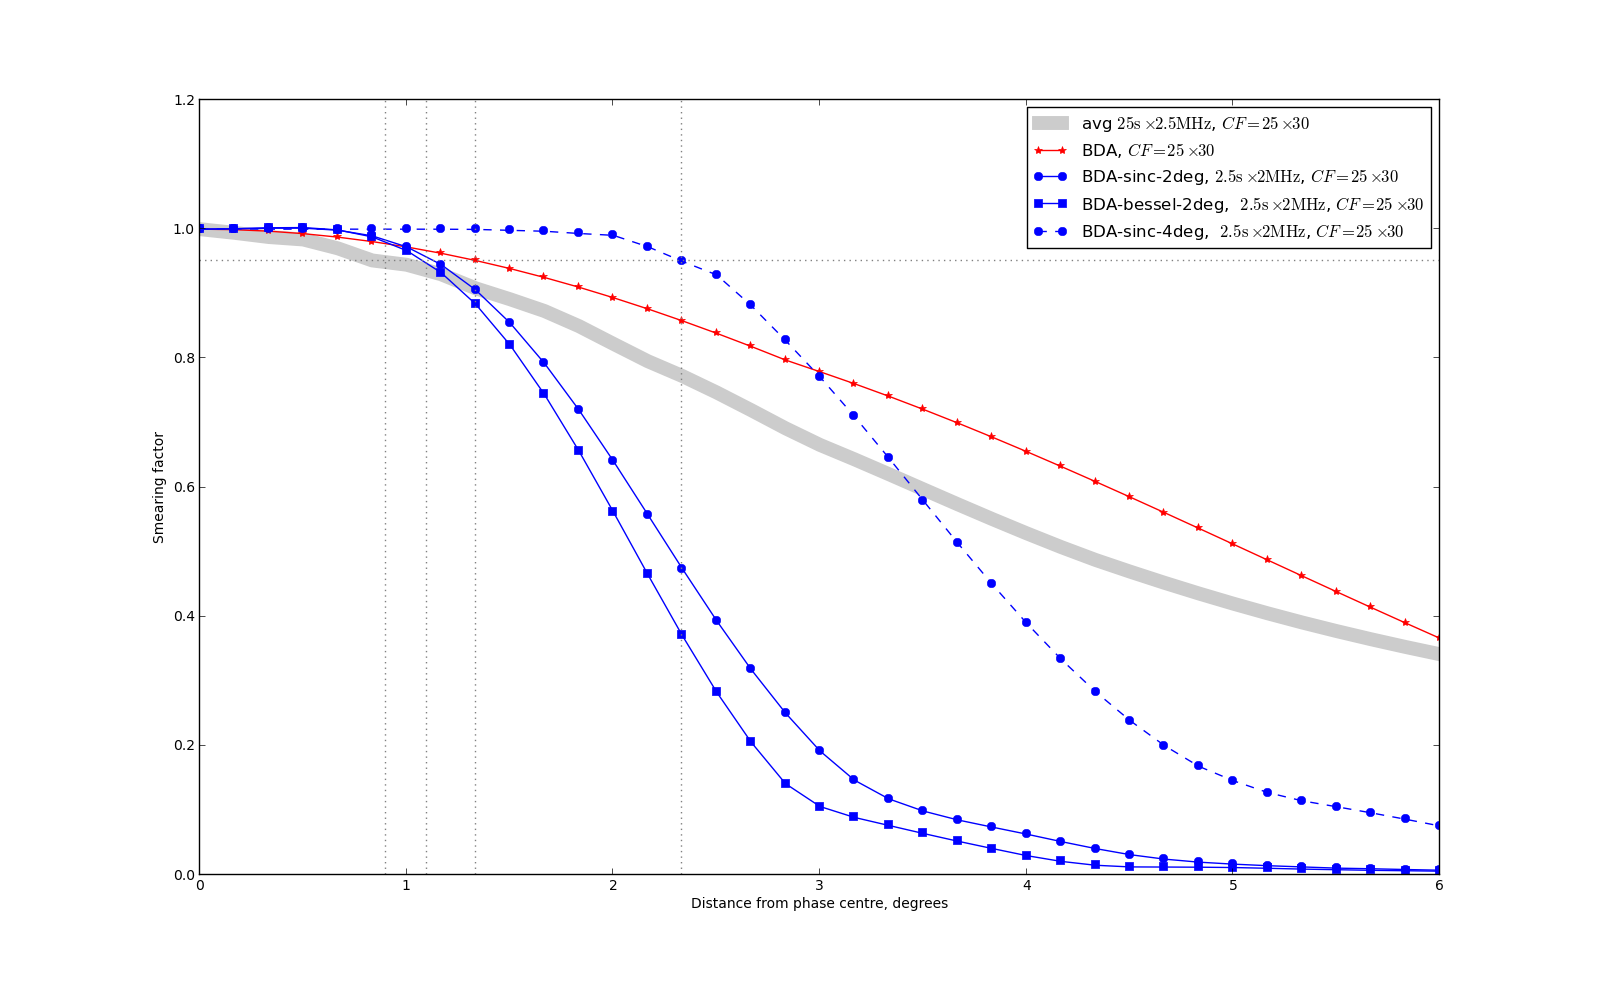
\includegraphics[width=1.2\textwidth, angle =90]{./Figures/suppression-25-2-5MHx-bda.png}
\caption{Amplitude loss: the apparent intensity of a 1 Jy source as seen by JVLA-C at 1.4 GHz as a function of distance from phase centre, for simple averaging with \BIN{25}{2.5} bins, and for BDA, and overlapping BDWFs for equal 
compression factor of $CF=25\times 30$.}\label{fig:bda-sn-bessel-2ge}
\end{figure}


\section{Conclusion}
 For a fixed time length a long baseline will cover a
longer track in visibility space compared to a shorter baseline which results in
the lower spatial modes being oversampled compared to higher spatial modes.
This necessitates the use of baseline-dependent averaging to optimize the
image plane response for each baseline. The use of baseline dependent 
averaging and BDWFs for an equal $uv$-space averaging have been investigated, this in two different aspects: 
mathematically and  via simulations.

We have identified and established that baseline dependent averaging 
can only be used for purpose of data compression and FoV recovering i.e baseline dependent averaging
decreases smearing over the observation FoV, while on the other hand, sources out of this field are 
not suppressed compared to simple averaging. 
We have found that combining BDA with BDWFs results to an  excellent tapering behavior,
which can decrease smearing to about $1\%$ or less over a selected  FoV, with  out of FoV sources suppression
almost two orders of magnitude higher compared to simple averaging, while the data is compress at the same rate.

We should also note that, baseline dependent averaging also distorts the PSF, and differently compared 
to simple averaging. An interesting avenue for future work is deriving this PSF at different sky position
for the case of baseline dependent averaging in the offing to integrate into  an existing imager.

We still have to keep in mind that, using baseline dependent averaging, the calibrations parameters as was described in
the introduction will change during the observation, due to the varying time and channel lengths on different baselines.
This is an obvious direction for future research plan with baseline dependent averaging. 


\bsp
\label{lastpage}
\end{document}
